


\chapter{ Experimental Setup} \label{ch:ExpUp}

\section{Thomas Jefferson Lab}
\paragraph{}Thomas Jefferson National Accelerator Facility(Jlab) in Newport News, Virginia hosted the MARATHON experiment in the Fall of 2017 and Spring of 2018. Jlab uses support from the U.S. Department of Energy(DOE) and the state of Virgina to complete the lab's mission of delivering productive research by exploring the atomic nucleus and its fundamental constituents, including precise tests of their interactions. Along with applying an advanced particle accelerator, particle detectors and other technologies to develop new basic research capabilities and to address the challenges of a modern society.
\subsection{CEBAF}\label{sec:cebaf}
	\paragraph{}The Continuous Electron Beam Accelerator Facility (CEBAF) was recently upgraded to a 12 GeV accelerator. The upgrade allows the accelerator to deliver a 11 GeV beam of continuous electrons of up to 200 $\mu$A of current to three experimental halls (A,B,C) and 12 GeV to the recently constructed hall D. 
\subsection{Injector}
	\paragraph{} CEBAF uses a micro-pulsed structure from the photo-electron gun to produce electrons in an efficient manner. This micro-pulsed structure is used to prolong the lifetime of the photocathode. The delivery of unique current and energy to all four halls requires the micro-pulses to have a 250 MHz or 500MHz structure and four individually tuned lasers. Frequencies of 250 MHz and 500MHz are chosen because these are sub-harmonics of the fundamental accelerator operating frequency of 1500 MHz. 
	\begin{figure}[t]
	\centering
	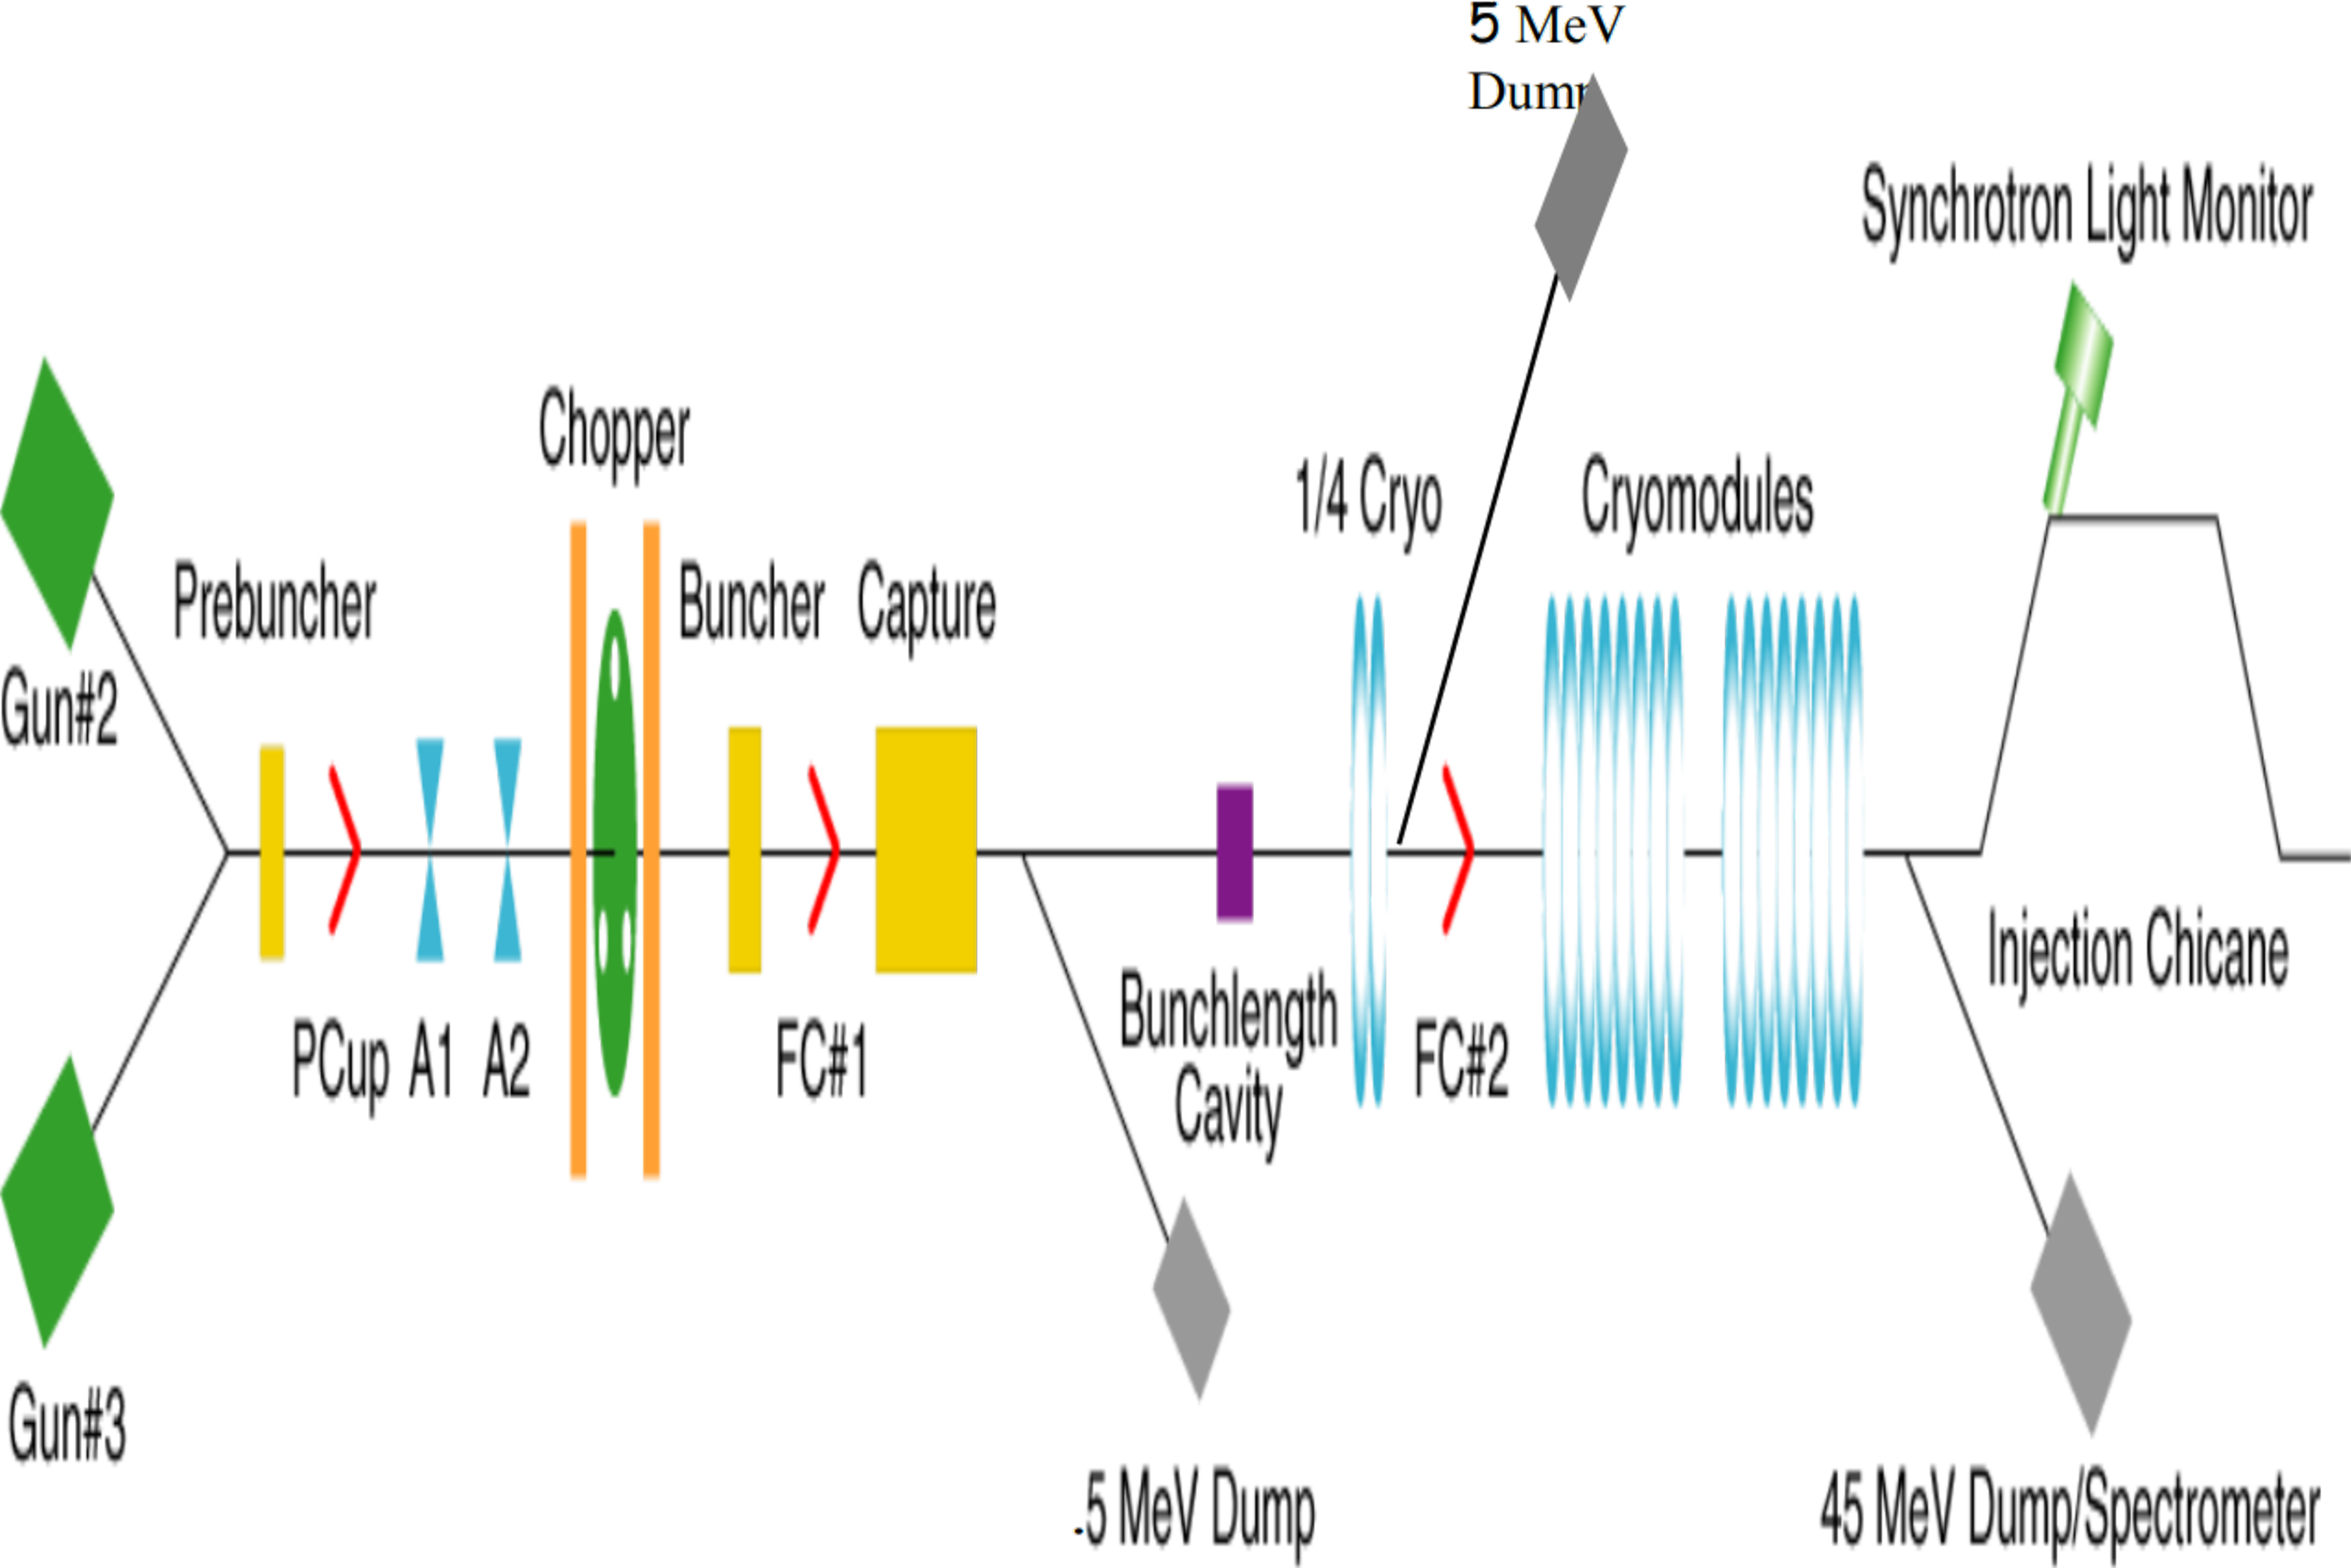
\includegraphics[width=12cm]{injector.pdf} 
		\caption{Drawing of the Injector layout. }
	\label{fig:inj}
	\end{figure} 
	\paragraph{}Electrons are produce when laser light shines on a gallium arsenide photo cathode. A laser pulse excites electrons from the photo cathode via the photoelectric effect. These exited electrons form from the gallium arsenide wafer when the electrons are excited out of the valence band into the conduction band. Gallium arsenide was chosen because the energy level of the conduction band for this photo cathode sits above the energy of an electron vacuum. Electrons in the conduction band escape from the material and accelerate away from the wafer due to high negative potential on the photocathode wafer \cite{sane}. 
	\paragraph{}Electrons that escape the photocathode wafer accelerate into the injector beam line due do the electron gun. Slits in the rotating chopper allow for regulation of the currents sent to the four experimental halls by reducing the number of electrons allowed through the chopper. Testing and calibration of the four beams are done throughout the injector beam lines via the Faraday cups located at different spots in the beam line. The polarized gun can supply electrons with up to 80$\%$ polarization and the polarization direction can be controlled by a wien filter. The level of polarization is ensured through measurements from a 5 MeV Mott polarimeter\cite{HallA}. The injector accelerates the electrons up to 123 MeV before allowing them into the north LINAC	\cite{ref:4beams,CEBAF,ref:photogun}.
\subsection{Accelerator}
	\paragraph{} Electrons travel through two LINACs and two bending arcs per complete pass of the accelerator. The two LINACs are approximately a quarter-mile long and are thirty feet below the surface. The beam lines are kept under vacuum between $10^{-6}$ and $10^{-11}$ torr to provided an efficient medium for transfer.  Electrons traveling to Halls A, B, and C complete a maximum of four and a half revolutions around the accelerator. These particles receive approximately 2.2 GeV in energy for each cycle through the accelerator. 
	\begin{figure}[h]
		\centering
		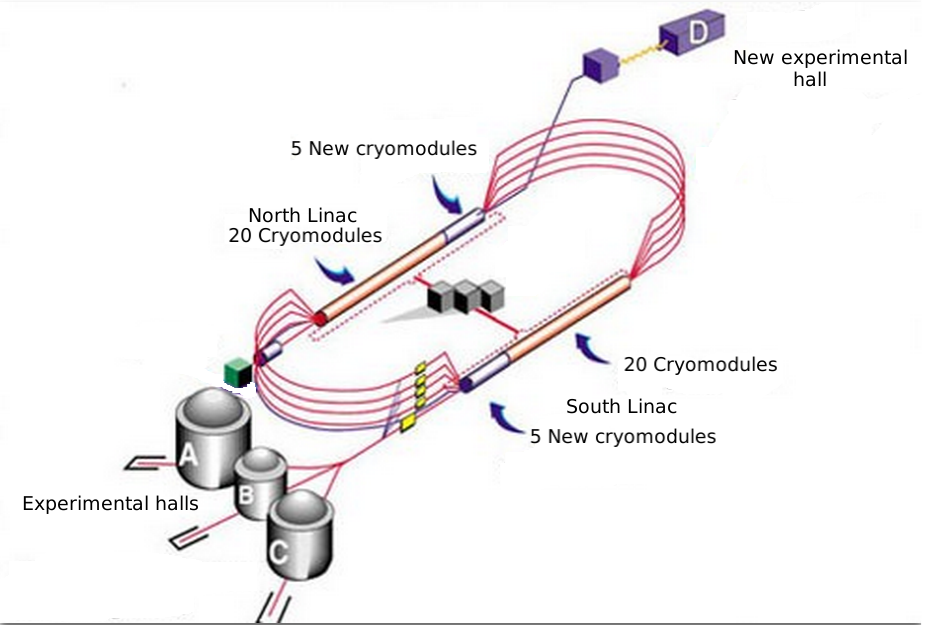
\includegraphics[width=12cm]{CEBAF.png} 
				\caption{Schematic Layout of CEBAF. }
		\label{CEBAF}
	\end{figure} 
	\paragraph{}The radio frequency (RF) cavities in each LINAC use an oscillating electromagnetic field to supply a force to accelerate the passing electrons. These Niobium RF cavities are cooled to 2 K to create conditions that allow the cavities to be superconducting \cite{HallA}. The superconducting RF(SRF) cavities provided a negatively charge field behind the electrons and positively charged field in front to accelerate the electrons through a set of cavities inside a cryomodule. A central helium liquefier circulates up to 17000 gallons of chilled liquid helium to control the temperature of the cryomodules. A dedicated 5 kW klystron  provides a 1500 MHz RF driving signal for each cryomodules. 
	\paragraph{} The electron beam exiting the north LINAC enters the east arc. The east and west arcs contain large dipole and quadrupole magnets to steer and focus the beam as it accelerates back to the other LINAC. After electrons exit the south LINAC, they either continue on around the accelerator for another pass to increase in energy, or a RF separator projects the electron beam into the proper experiment hall \cite{CEBAF}. Energy loss, beam position, and beam charge monitors lie throughout the beam line, and are used to ensure high quality beam delivery to the experimental halls. The accelerator staff in the machine control center(MMC) and the experimentalist in the experimental halls collaborate together to provide an atmosphere for safe and efficient scientific discovery.

 \section{Hall A Beam Line}\label{sec:halla}
	 
	\begin{figure}[H]
		\centering
		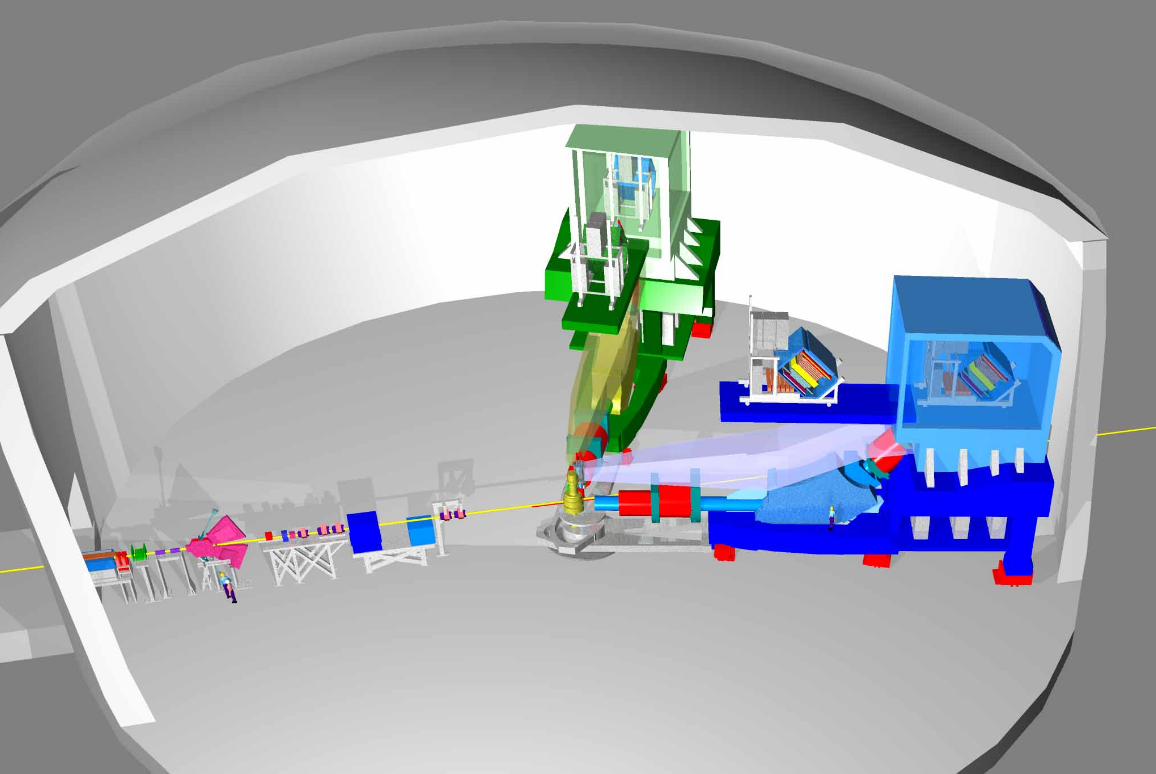
\includegraphics[width=12cm]{HallA_2.png} 
				\caption{A 3D drawing of Hall A. }
		\label{HallA}
	\end{figure} 	 
	 
	 \paragraph{}The experimental Hall A and the scientific equipment used were designed for detailed investigations of electro and photo-induced reactions. Two high resolution spectrometers in Hall A use the inclusive (e,e$\prime$) and exclusive (e,e$\prime$ p) reactions to gain a greater understanding of the structure of the nucleus. Completing detailed studies with high resolution and extreme accuracy requires knowing the beam position, size, energy, and current when the beam strikes the target. The instrumentation used in the precise measurement of these quantities in Hall A  are shown in figure \ref{BeamLine} \cite{HallA}. The information provided by these detectors originate through small changes in current and voltage sent through the electronics. Detector calibrations turn the signals from these detectors into useful information.
	 
	 \begin{figure}[t]
	 	\centering
	 	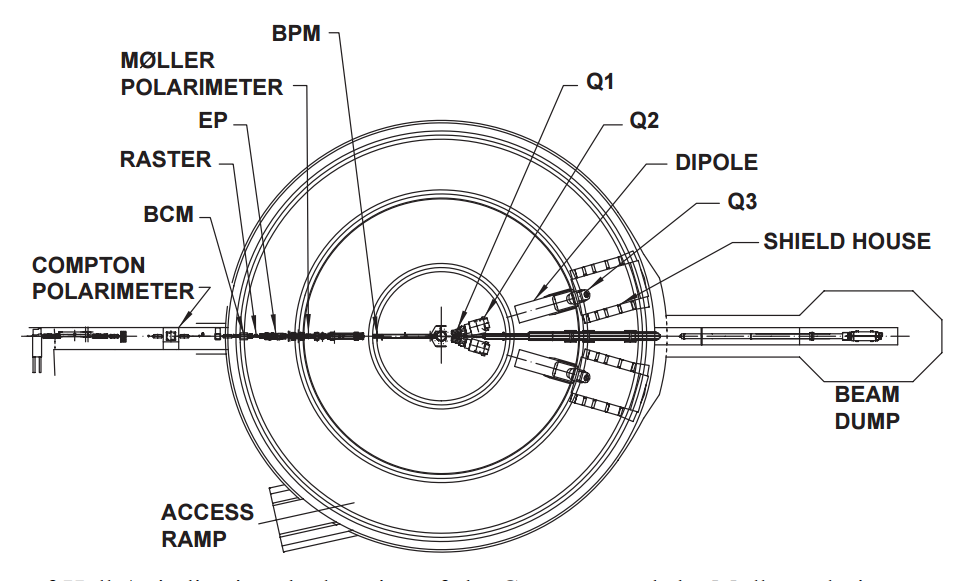
\includegraphics[width=14cm]{BeamLine.png} 
	 		 	\caption{A schematic layout of the beam line in Hall. \cite{HallA} }
	 	\label{BeamLine}
	 \end{figure} 	
	 
 
	 \subsection{Beam Position Monitors}
	 \paragraph{} A pair of Beam Position Monitors(BPM)s measure the relative beam position without affecting the beam. The two Hall A BPMs are located at 7.524 m and 1.286 m away from the target. Using the standard difference-over-sum technique, the relative beam position is determined with an accuracy of 100 $\mu$m with a beam current of at least 1 $\mu$A \cite{HallA}. The BPMs' positional data is recorded in two ways. Every second of beam time, the beam position average over 0.3 seconds is logged into the Experimental Physics and Industrial Control System (EPICS) database. The BPMs also transmit data event-by-event to the CEBAF online Data Acquisition system(CODA).
	 	 	 

 \paragraph{} The main beam line components of the BPMs consist of four open-ended antennas. Figure \ref{BPMimg} shows a side view of a BPM chamber and figure \ref{BPM_4} shows the layout of the four antennas as you look down the beam line. The antennas are titled $u_+$, $u_-$ and $v_+$, $v_-$. The antennas receive an induced signal as electrons pass to determine the beam position in the u and v directions. The BPMs send a DC offset to the DAQ. This DC offset is turned into a positional measurement via an ADC calibrated signal. The position of one axis is determined through the difference over sum method:
 \begin{equation}
 	u = \frac{u_+ - u_-}{u_+ + u_-}.
 \end{equation} 
  	\begin{figure}[H]
 	\centering
 	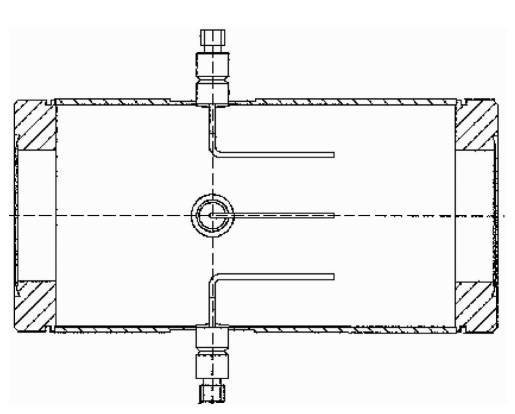
\includegraphics[width=12cm]{BPM.png} 
 	\caption{BPM design diagram, from JLab instrumentation	group. Beam direction is from left to right \cite{BPM2}. }
 	\label{BPMimg}
 	\vspace{1.5cm}
 	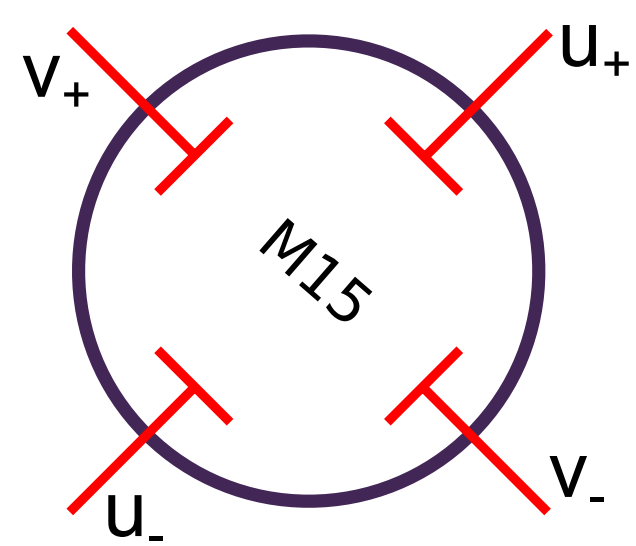
\includegraphics[width=10cm]{BPM_4.png}  	
 	\caption{BPM design diagram, looking down the beam line\cite{BPM2}. }
 	\label{BPM_4}
 \end{figure} 
  
 
 The beam position in the frame of the u and v antennas are calculated by the taking the difference over the sum of the two wires in the u and v directions. The accuracy of the BPMs requires an absolute measurement of the electron beam's position to calibrate the BPMs\cite{BPM,BPM2}.

\paragraph{} Figure \ref{harp} shows an image of the harps used for BPM calibration. Each harp is located immediately after the BPM on the beam line. The harp forks are aligned perpendicular to the beam line to allow the harps to move in and out of the beam line. A wire that traverse between the fork tines at three different angles in respect to the harp detects electrons passing through the beam line. The two sloped sections of the wire are angled at 45$^{\circ}$ relative to the harp frame. As the harp fork moves into the beam, the wires receive a signal as the beam interacts with the wires. The signal strength from the harp wire represents how close the wire is to the beam. A peak in the signal demonstrates the location of the beam in respect with the corresponding wire. The two sloped wires are used together to determine the vertical position of the beam. The vertical wire is used to determine the horizontal position of the beam \cite{BPM,BPM2}. The harps are not used during production phases due to their intrusive nature caused by the interaction of the beam with the harp wire.
		\begin{figure}[t]
			\centering
			\caption{A schematic layout of a harp fork \cite{BPM2} }
			\label{harp}
			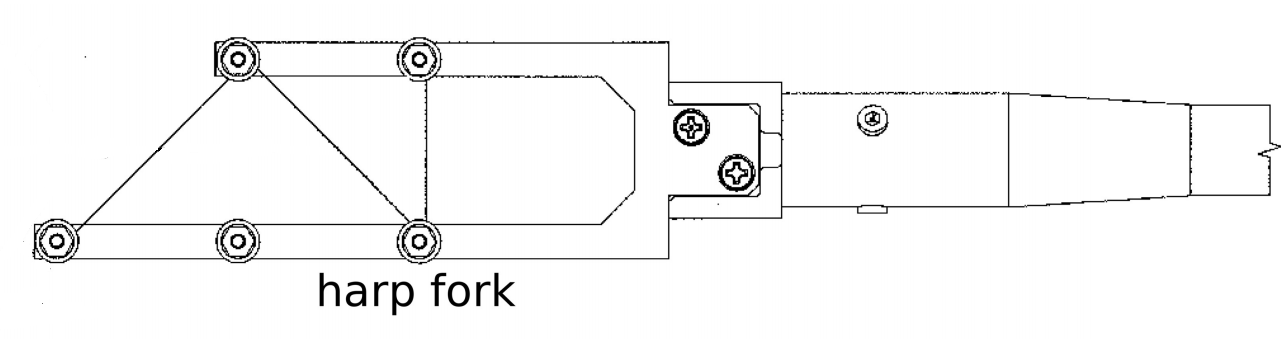
\includegraphics[width=14cm]{harp.png} 
		\end{figure}  	
		
		\paragraph{}The location of the wires on the harp frame and the position of the harp fork were used to calculate the absolute beam position. Figure \ref{bullsB} shows an example of five positions used to calculate the BPM calibration coefficients and the BPM position reading before calibration. This method of using beam positions at the nominal center and surrounding the center is called a bull's eye scan. The harp scan results are substituted into equation \ref{BPM_eq} for the X and Y positions. Using all five points and an $R^2$ regression technique, the coefficients can be determined with great accuracy. Figure \ref{bulls} shows the comparison between harp position and BPM after calibration. These highly accurate BPMs were crucial in reducing systematic error in the final results obtained from this experiment. 
		\begin{equation}
		\label{BPM_eq}
		\begin{pmatrix}
		X_{position}\\
		Y_{position}
		\end{pmatrix}
		=
		\begin{pmatrix}
		C(0,0) & C(0,1)\\
		C(0,0) & C(0,1)\\
		\end{pmatrix}
		*
		\begin{pmatrix}
		X_{BPM}\\
		Y_{BPM}
		\end{pmatrix}
		+
		\begin{pmatrix}
		X_{offset}\\
		Y_{offset}
		\end{pmatrix}			 
		\end{equation}
		
		\begin{figure}[H]
			\centering
			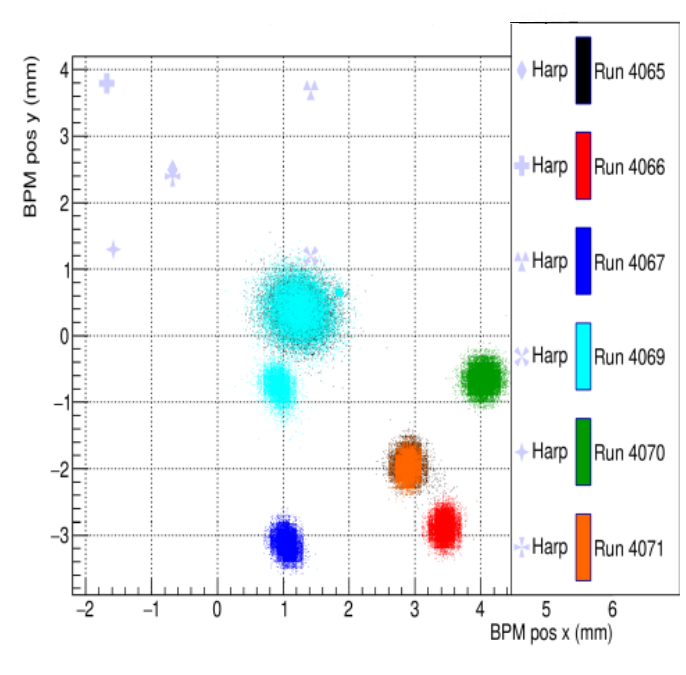
\includegraphics[width=9.5cm]{BPM_before.png} 
			\caption{The X and Y position comparison for harp to BPM for a bulls eye scan before BPM calibration. }
			\label{bullsB}

			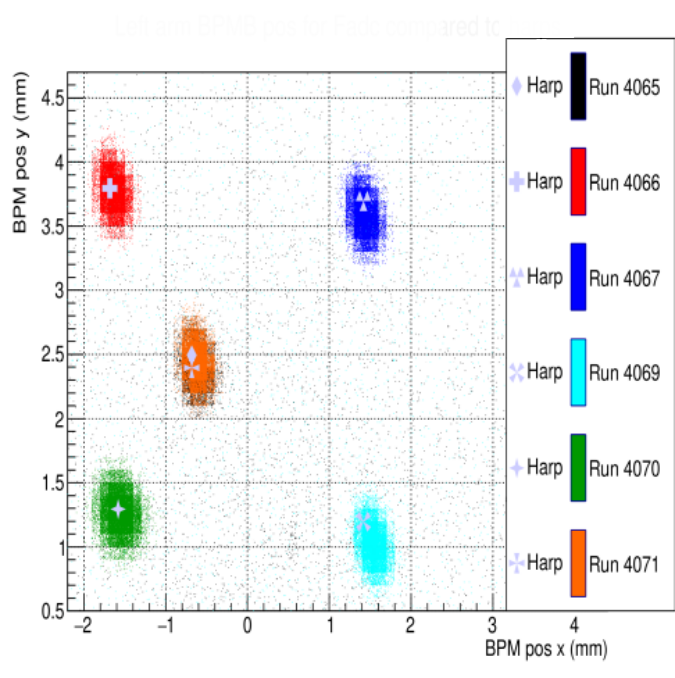
\includegraphics[width=9.5cm]{BPM_after.png} 
			\caption{The X and Y position comparison for harp to BPM for a bulls eye scan after BPM calibration. }
			\label{bulls}
			
		\end{figure} 	

	 \subsection{Raster}
	 \paragraph{} Damage to a target system from intense beam can cause extreme fluctuations in the target's temperature and density. A raster was used to counteract the damage caused by a focused beam. The raster used two magnetic fields produced by two dipoles to spread the electron beam out. This produces a large rectangle interaction area on the front face of the target container. A triangle wave of 25 kHz controls the coils of the dipole magnets. The raster system begins $\approx$17 meters before the target chamber\cite{BPM2}. The raster system's relative position can be seen in figure \ref{HallA}. Safety constraints administrated by the target group at JLAB limited the minimum size of the raster spot for the MARATHON experiment to two millimeters by two millimeters. The 2x2mm minimum limit for the raster size was installed as a preventative safety measure to eliminate concerns breaking containment of the $^3$H target through damage to the entrance window. 
	 \paragraph{} The Hall A raster system consists of four dipoles. Two dipoles produce magnetic fields in the horizontal direction of the lab frame and two in the vertical. The upstream raster and downstream raster include one vertical and one horizontal dipole. The relative change in position of the incoming electrons are controlled by the current supplied to the dipoles. This current that drives the dipoles is recorded by an ADC. In order to obtain the change in beam position due to the raster, a calibration between the raster current and measured beam position were obtained.  
	  \begin{figure}[th!]
	 	\centering
	  	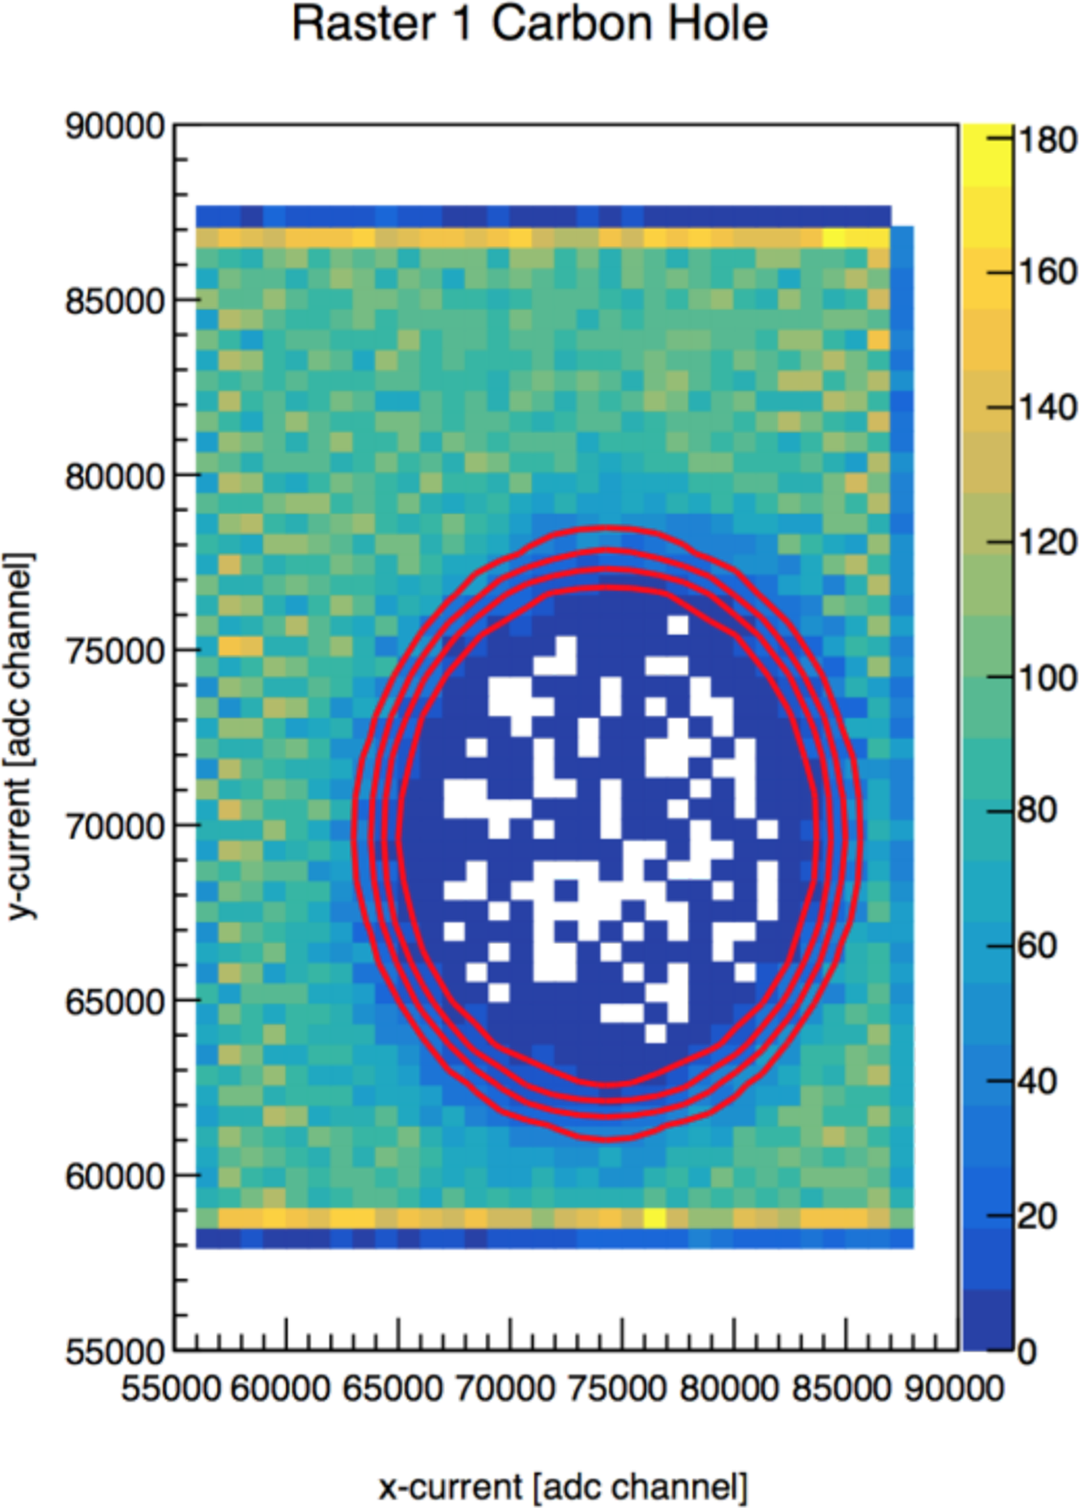
\includegraphics[width=7.5cm]{raster.pdf} 
	 	\caption{The X and Y current of the raster with a carbon hole. The size of the carbon hole is fit with a radial sigmoid\cite{Trast}.}
	 	\label{fig:raster}
	 \end{figure} 
	 \paragraph{}
	 The raster calibration is done by creating a line that maps the raster current measured by ADC channels to a position. This calibration process is done to extract beam positions at the locations of both BPMs and the target center along the beam line. Calibrating the raster requires two calibration procedures. The first process was to determine the size of the rastered beam spread. In order to accurately determine the width and height of the beam spread due to the raster, a carbon foil with a hole of a diameter of 2mm was used. Events will only scatter from outside of the hole. Plotting the x and y raster current of the rastered beam will show the hole through a vacancy of events. The fit of the carbon hole gives the width of the raster, the slope of the linear mapping term. In figure \ref{fig:raster}, the raster current in x and y directions are fitted using this radial sigmoid. Once the slope of the linear calibration is determined, the offsets can be found. This is discovered by using the calibrated BPM mean positions for a phase of rastered beam. The mean positions for both BPMA and BPMB produce a track from the BPMs to the target. This projection provides a mean location of the beam at the target.  Using equation \ref{eq:raster}, the offsets also know as the intercepts are solved for using the slope ($m_x,m_y$), the raster mean current value ($R_x,R_y$), and the mean BPM position($x,y$) \cite{Trast}.
	 \begin{equation}
	 	\begin{pmatrix}
		 	x\\
	 		y
	 	\end{pmatrix}
	 	=
	 	\begin{pmatrix}
	 		R_x\\
		 	R_y
	 	\end{pmatrix}
	 	*
	 	\begin{pmatrix}
			m_x && 0 \\
			0  && m_y
	 	\end{pmatrix}
	 	+
	 	\begin{pmatrix}
		 	O_x\\
	 		O_y
	 	\end{pmatrix}
	 	\label{eq:raster}
	 \end{equation}

 
	 \subsection{Beam Energy}
	 \paragraph{}The electron beam energy is located in many of the equations used in an electron scattering experiment. This can cause a noticeable increase in systematic error if the beam energy measurement is not made precisely. In Hall A, the beam energy was measured by using the (e,e$\prime$p) method. On the beam line, 17 meters upstream from the target an ep scattering chamber is located. MMC directs the beam into the ep scattering chamber containing a rotating 10-30 $\mu$m thick tape of C$H_2$. The scattering angle of the electron and the recoil angle of the proton are used to determine the beam energy using equation \ref{EP}. Where $M_p$ is the mass of the proton and $\theta_p, \theta_e$ are the scattered angle of the proton, electron respectively. 
	\begin{equation}
	\label{EP}
	E = Mp \frac{cos\theta_e + \frac{sin\theta_e}{tan\theta_p}-1}{1 - cos\theta_e} 
	\end{equation}
	The beam energy was also measured using the ark measurement method \cite{Flay}. This method uses changes is beam position and precise measurements of the magnetic fields around the beam line to determine the energy of the electron beam. The angle at which the electrons bend through the magnetic field relates to the momentum of the electrons,
	\begin{equation}
	\label{arc}
	p = k \frac{\int \vec{B} \cdot d\vec{l}}{\theta}.
	\end{equation}	
	In equation \ref{arc}, p is the momentum of the electrons, $\theta$ is the bend angle, and $\vec{B}$ is the magnetic field the electrons experience. Then using the momentum of the electron, the energy of the beam can be extracted. The error on the beam energy measurement is $\delta$ E/E $\approx$ 2 $* 10^{-4} $ \cite{EPMet, Flay}.  The MARATHON experiment used both methods to accurately determine the electron beam energy.
	
		  	\begin{figure}[t]
		  	 	 		\centering
		  	 	 		\caption{Hall A Current Monitor components \cite{BCM1}. 
		  	 	 		\label{BCMpng}}
		  	 	 		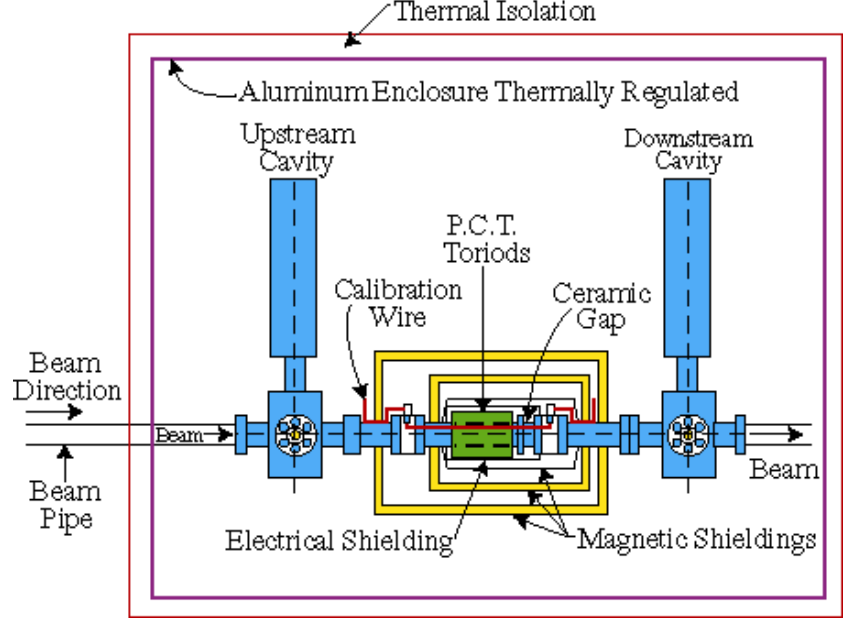
\includegraphics[width=10cm]{BCM1.png} 
		  	\end{figure}
	\subsection{Beam Current Monitors}
	\paragraph{} The main process of measuring the scattering yield for a calculation of a cross section looks at finding the ratio of the number of electrons scattered to the number of electrons sent. In order to accurately determine the number of electrons sent to scatter with our target system, Hall A use a set of non-invasive beam current monitors(BCMs). The Hall A BCMs have an absolute accuracy of 0.2 percent as long as the current is between 1 and 180 $\mu$A. The BCMs used in Hall A consist of three main components: a Parametric Current Transformer (PCT) and two pill box cavities. Figure \ref{BCMpng} shows the components in the Hall A BCM.  The BCM produces an RF signal that is proportional to the beam current. A 10 kHz down converter, RMS-to-DC converter, voltage-to-Frequency converter, and a scaler convert the are used to inject the current signal into the Hall A DAQ. Proportionality constants are determined in the calibration process to correctly integrate the charge for a given amount of beam current\cite{BCM1}.
	\begin{figure}[t]
		\centering
		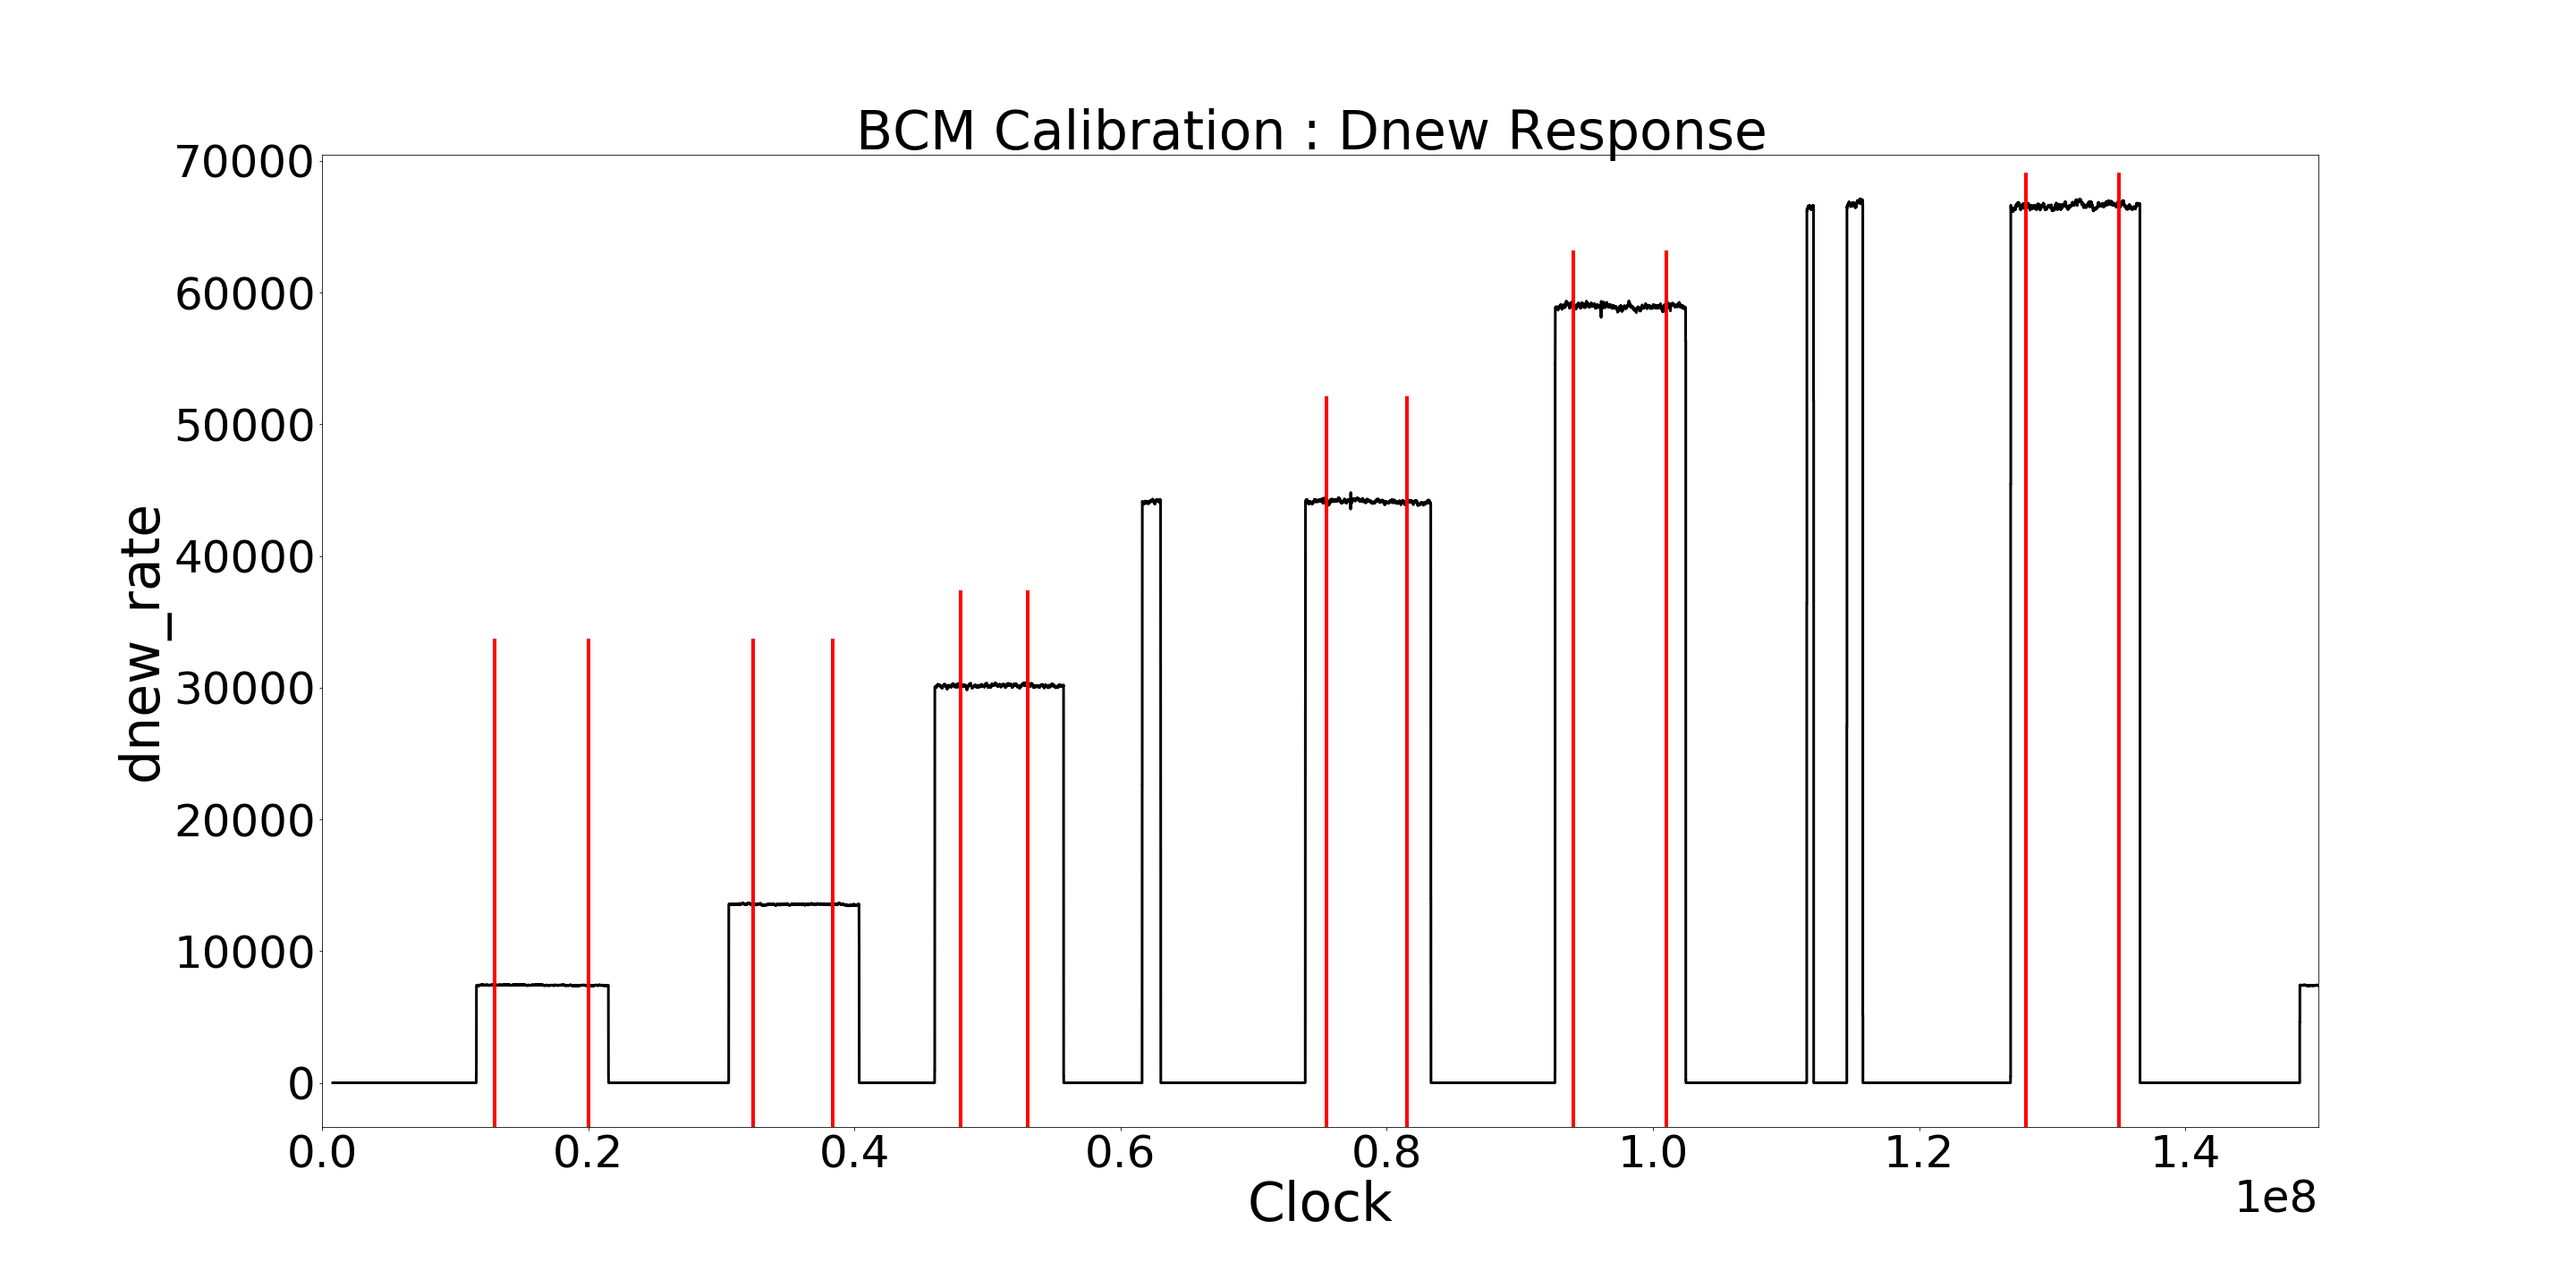
\includegraphics[width=17cm]{dnew_freq.png}
		\caption{BCM calibration, changing the current at observing the rate \cite{MikeTh}.
		\label{dnewfreq}}
	\end{figure}
	\paragraph{}The process of calibrating the BCM converts the frequency received from the BCMs to an amount of current in $\mu$A. In order to calibrate the BCMs in Hall A, a separate intrusive calibration of an unser must be done. The unser is calibrated by inserting a known current through a wire inside the beam pipe. The calibration of the unser is known to drift over time, which makes the unser unfeasible to use as the main source of charge calculation. Once the unser is calibrated, the BCM calibration procedure can be completed. The BCM calibration requires the delivery of the electron beam with unique procedure. This process consists of oscillating the beam on and off status while increasing the current. Figure \ref{dnewfreq} shows the process of alternating current on and current off at different magnitudes of current. This stepping up procedure provides an adequate number of data points to complete a linear fit of the BCM frequency verses the calibrated unser current. The linear fit parameters supply a multiplicative gain and an additive offset for the calibration of the BCMs. Figure \ref{bcmcal} shows a linear fit that provides gain and offset calibration constants for the BCM used in the calculation of charge. 
	\begin{figure}[t]
		\centering
		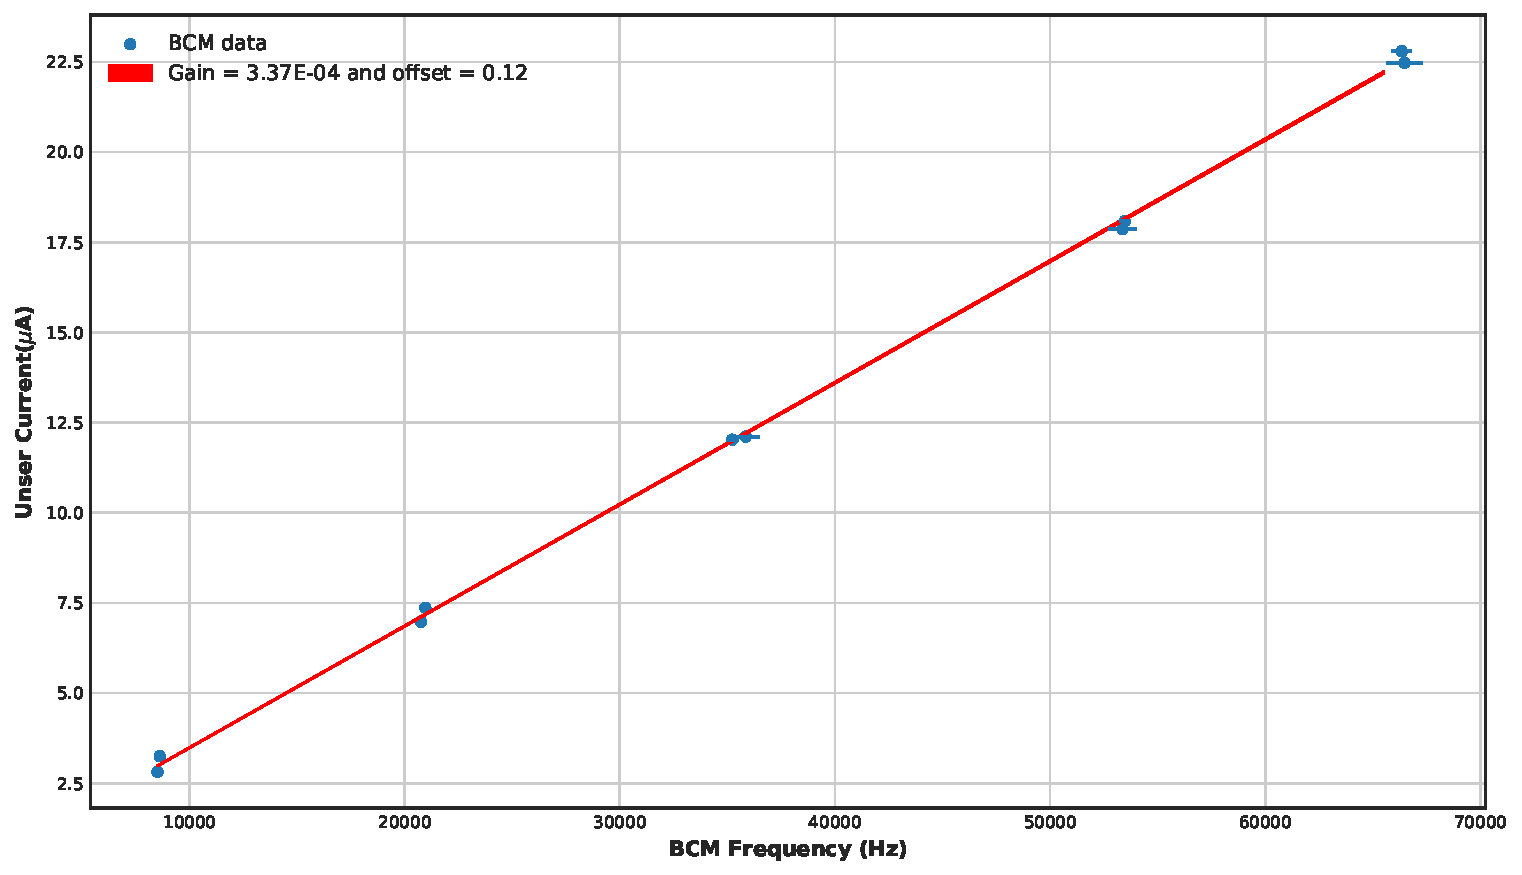
\includegraphics[width=15cm]{BCMcal.pdf}
		\caption{The relationship between unser current and BCM frequency for BCM calibration \cite{MikeTh}.
			\label{bcmcal}}
	\end{figure}	
	  
\section{Target}\label{sec:target}
\paragraph{} The $^3$H run group of experiments, including MARATHON, used the newly designed Hall A $^3$H Target(HATT) system. The HATT target chamber was repurposed from a previously used cryogenic target chamber to reduce the financial cost of designing a new target chamber. The refurbishing of the cryogenic target chamber consisted of adding in new safety features to prevent and mitigate a $^3$H leak.  A 4 inch long collimator with an inner diameter of 0.4 inch was added inside of the target chamber upstream of the target ladder to prevent the beam from striking the thin side wall of the aluminum cell. In case of a $^3$H leak in the target chamber, an exhaust system was installed to control the amount of $^3$H exposed to the Hall.\cite{HATT_eng}  Figure \ref{HATT} shows the HATT system with the target ladder in the home position and the scattering windows removed. 
\begin{figure}[t]
	\centering
	\caption{Target Images}
	\hspace*{-20pt}
	\subfloat[A image of the HATT. \cite{DHimages}]{{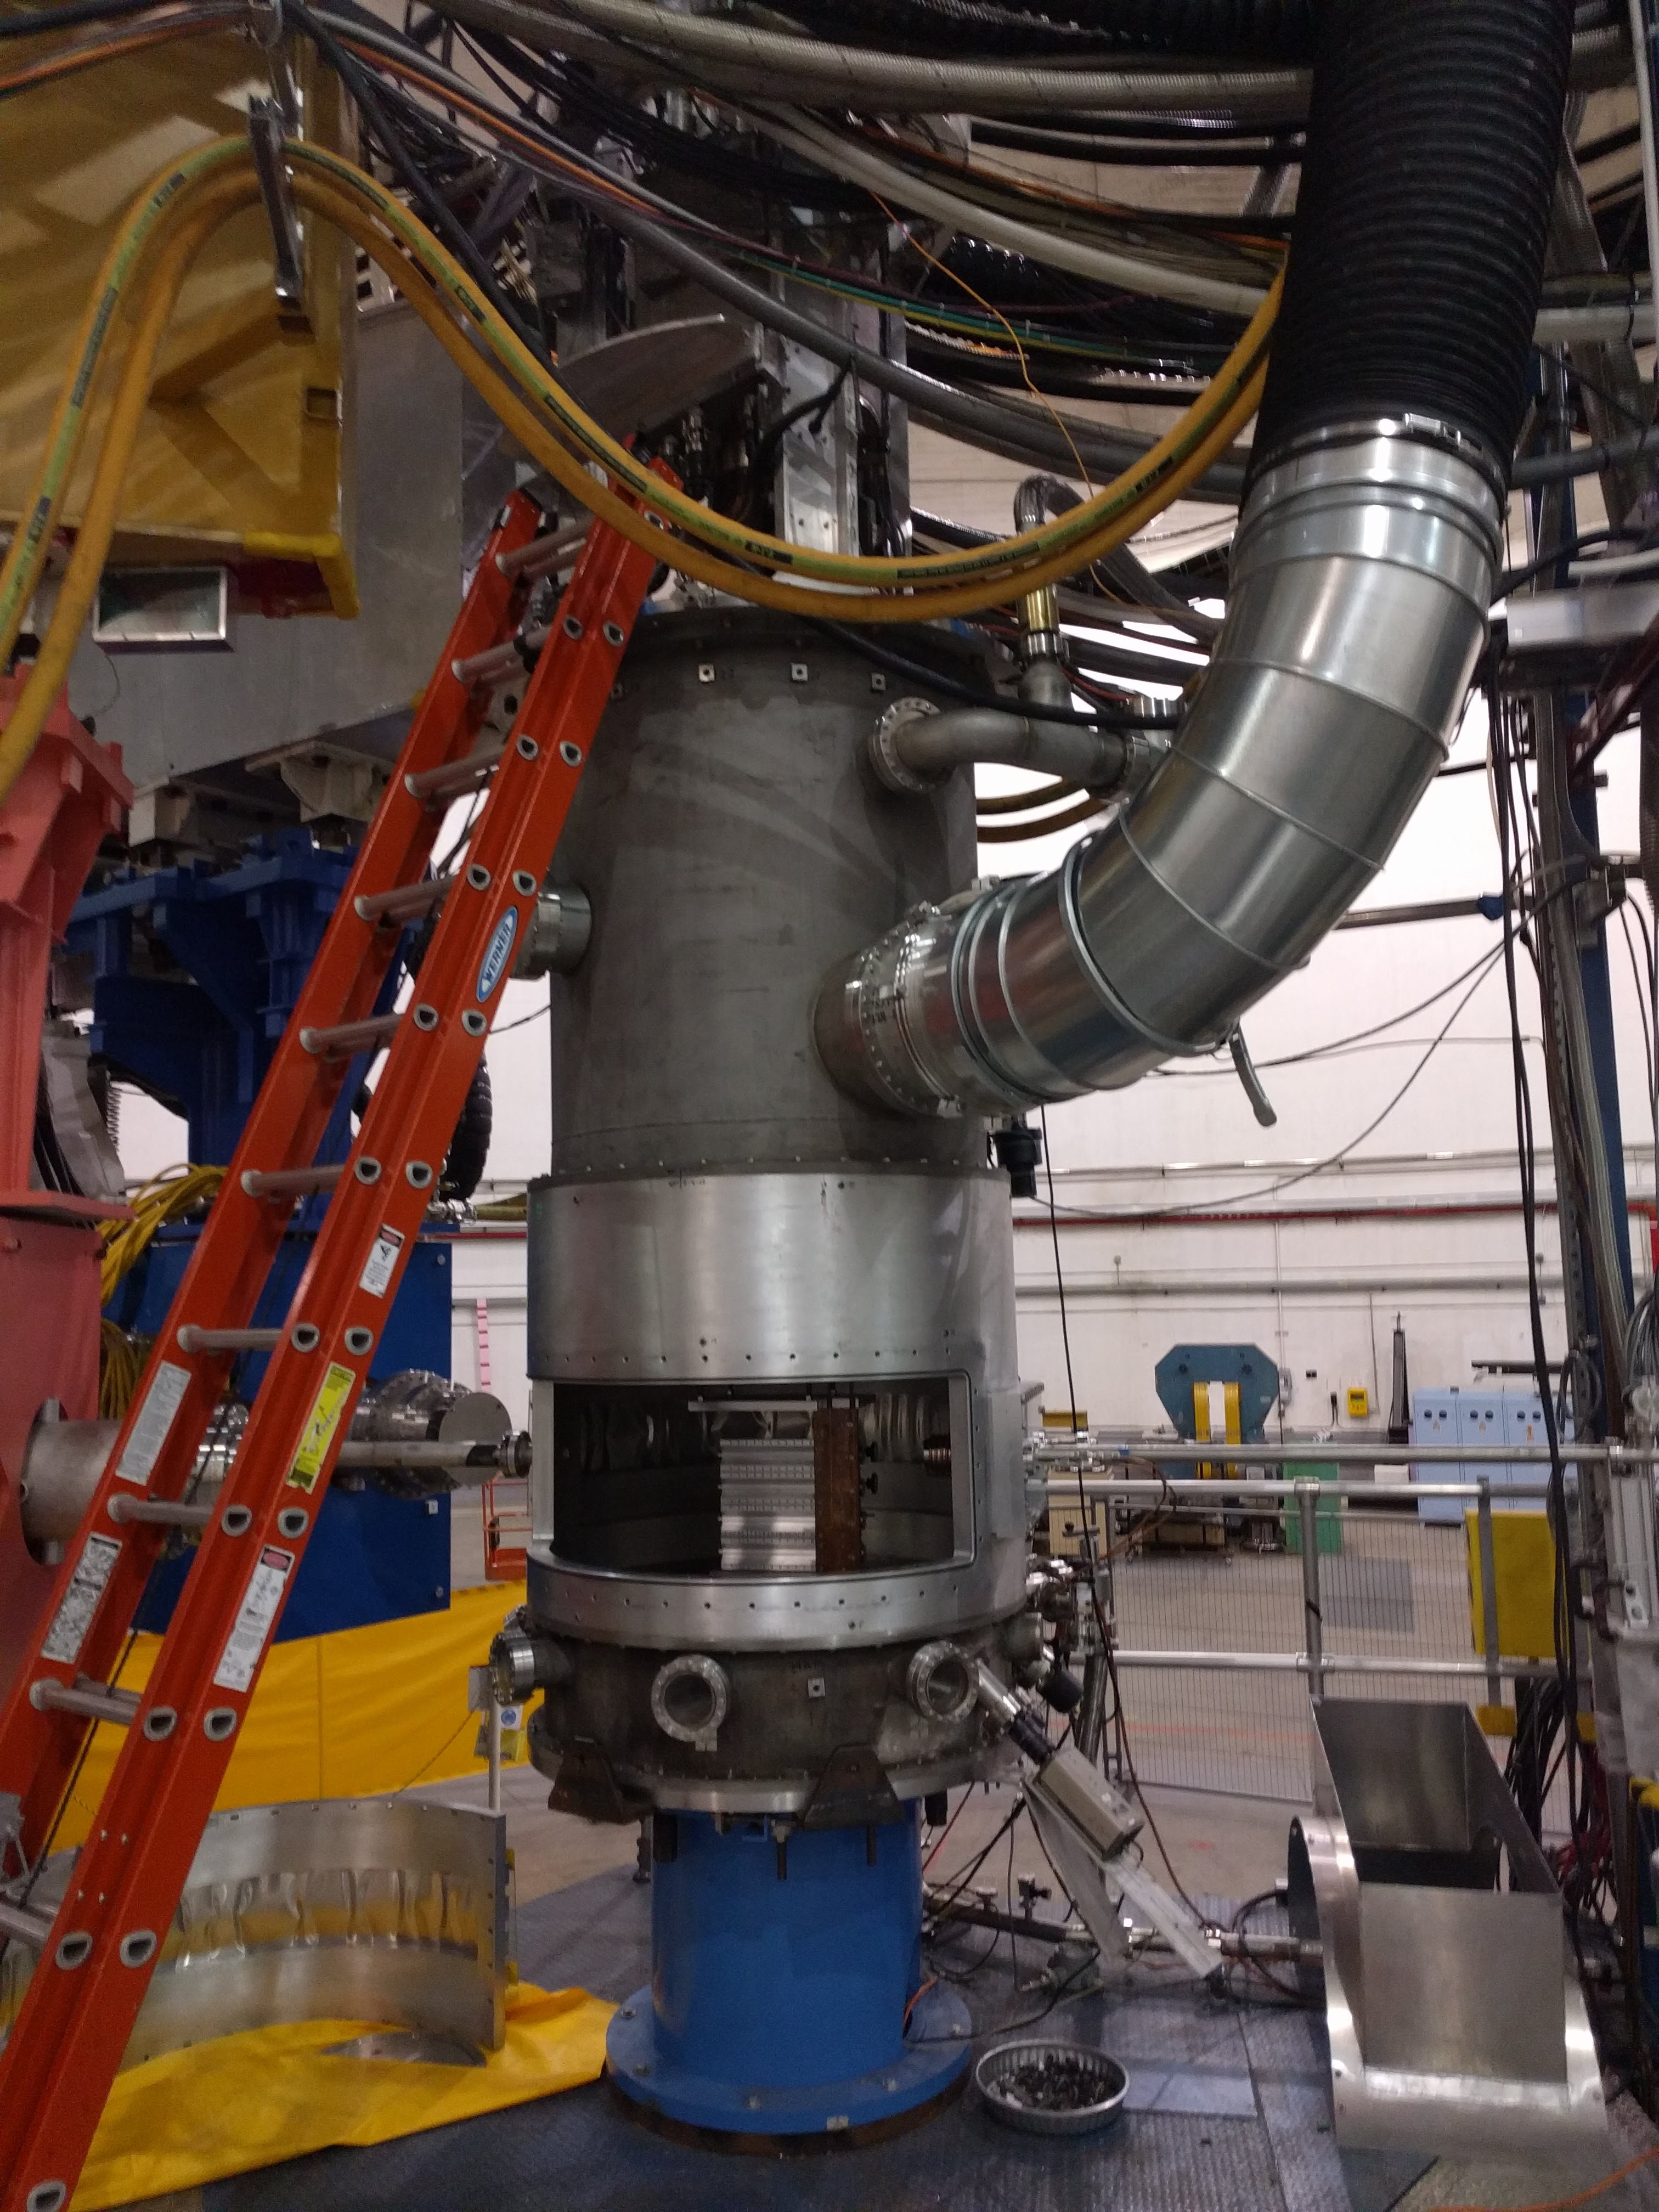
\includegraphics[width=6cm]{HATT.jpg} }}
	\centering
	\subfloat[Image of the Hall A $^3$H Target Ladder. \cite{DHimages}]{{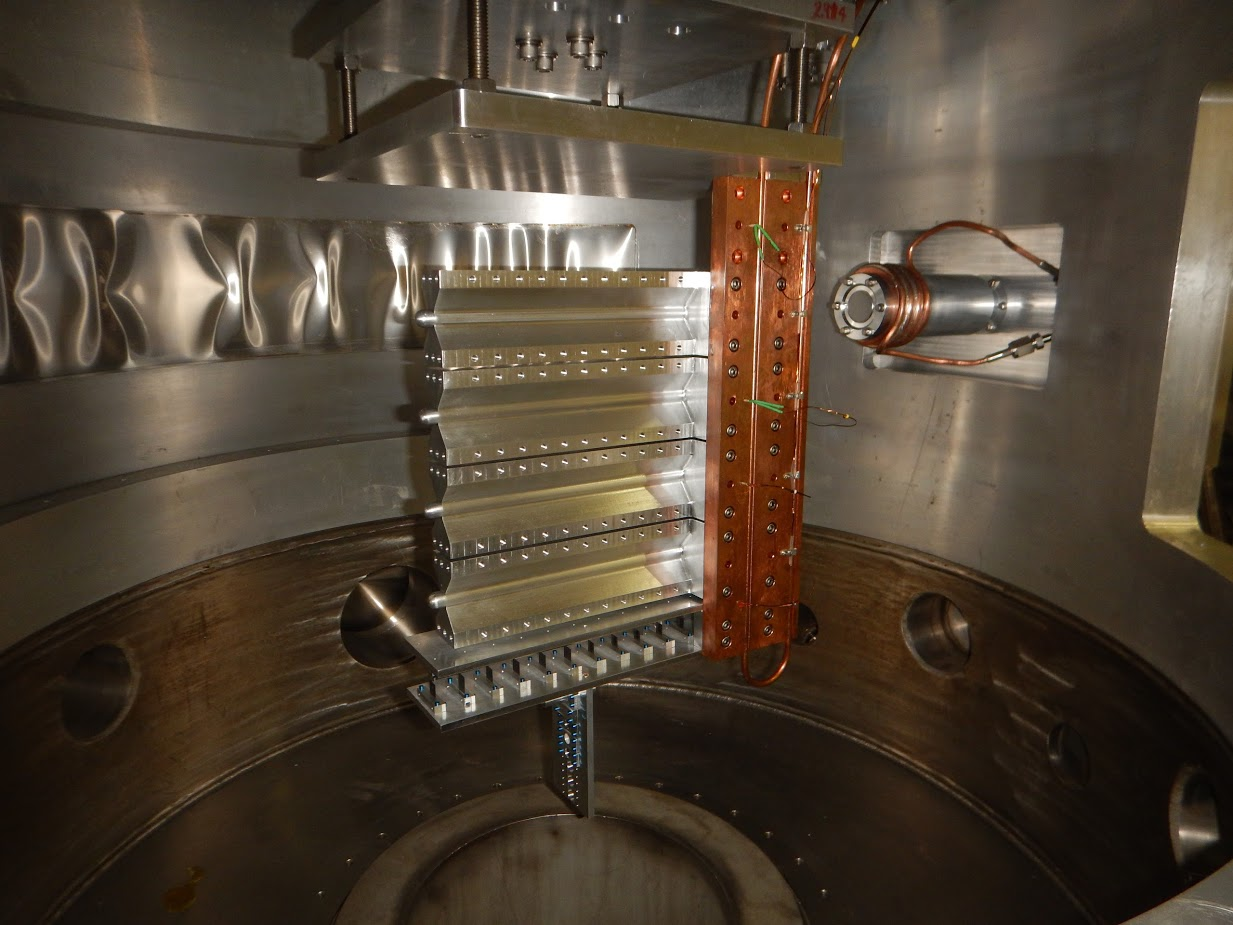
\includegraphics[width=8.5cm]{HATT_Ladder.JPG} }}
	\label{HATT}


\end{figure}
A picture of the HATT ladder installed in the HATT system is shown if figure \ref{HATT}. The ladder contains both gaseous cells and solid targets. The MARATHON experiment had five gas cells. The top four of the gas cells were filled with $^3$H3, $^2$H, H, and $^3$He3, from top to bottom. Due to safety restricts the $^3$H cell was not installed until the HATT system could be closed. The bottom most cell was left empty, to complete end cap subtraction. The lower half of the target ladder contains the solid targets used during the MARATHON experiment. The target cells are mounted to a heat sink with flowing cryogenics for temperature control of the target cells. Listed from top to bottom, the solid targets used were a pair of thick aluminum foils, carbon multifoil, single carbon foil, and a carbon foil with a 2mm diameter hole. The thick Al foils were used to aid the target window background subtraction. The multifoil target also know as the optics target was used to calibrate the z-axis  reconstruction of the optics matrix. The single carbon foil and carbon hole were used to calibrate the BPMs and raster and to determine the off set of the central line of the detector. 

\begin{figure}[t]
	\centering
	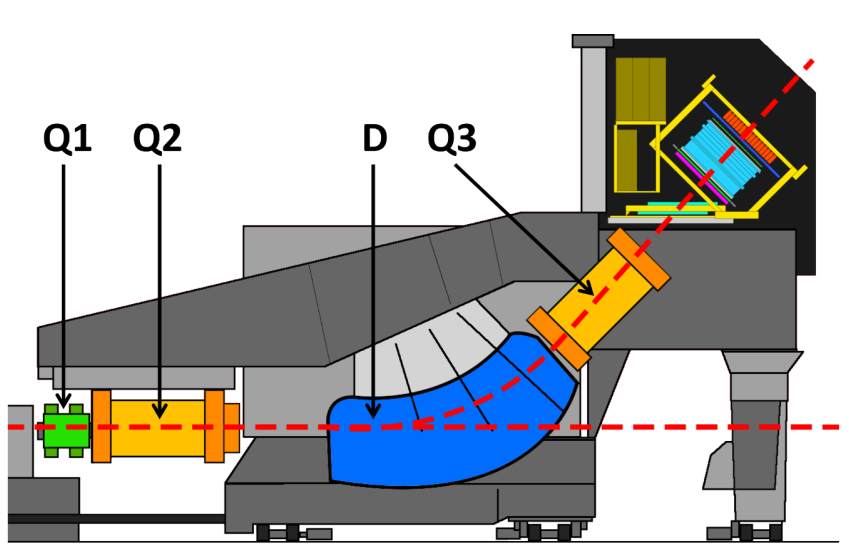
\includegraphics[width=10cm]{HRS_full.png}
	\caption{A side view of a HRS \cite{HallA}.
		\label{hrsfull}}
\end{figure}

\section{High Resolution Spectrometers}\label{sec:HRS}
\paragraph{}
Electrons that successfully scatter from the target may end up in either of the two HRSs(High Resolution Spectrometers). The HRSs were designed to detect charged particles with a high degree of precision. 
In order to achieve a high level of resolution in momentum and angle, the design of the HRSs consist of a magnet configuration of QQ$D_n$Q (quadrupole, quadrupole, dipole, and quadrupole). The vertical bending dipole provides the field required to transport the scattered particles through the 45$^\circ$ bending angle to the detector hut. A drawing of an HRS can be seen in figure \ref{hrsfull}. The first quadrupole(Q1) focuses the incoming electrons in the vertical plane. The following two quadrupoles (Q2 and Q3 provide transverse focusing. This optical design allows the use of extended gas targets with no substantial loss in solid angle\cite{HallA}.  
\paragraph{}The spectrometer's design allows for the performs of various functions which include: triggering the data acquisition system (DAQ) when certain requirements are met, gathering the position and direction of individual particles to reconstruct a track, provide precise timing information for time of flight calculations, and identify many different particle types that pass through the detector system. In order for both the Left HRS (LHRS) and Right HRS (RHRS) to  complete the required task, they contain a myriad of detectors. The HRSs use drift chambers, scintillators, Cherenkov detectors, and shower calorimeters. Both the Left and Right HRSs contain two planes of scintillators to function has the main trigger for the detector package. The vertical drift chambers (VDC) that lay at the front of the detector in conjunction with the Shower that lies in the back of the detector provide information for reconstructing the particle tracks and precise timing. Particles are identified by the Cherenkov, shower calorimeters, and pion rejectors that live in the left or right HRS. The layout of the individual detectors that make up the left and right detector package are shown in figure \ref{hrsss}  \cite{HallA}.
\begin{figure}[t]
	\centering
	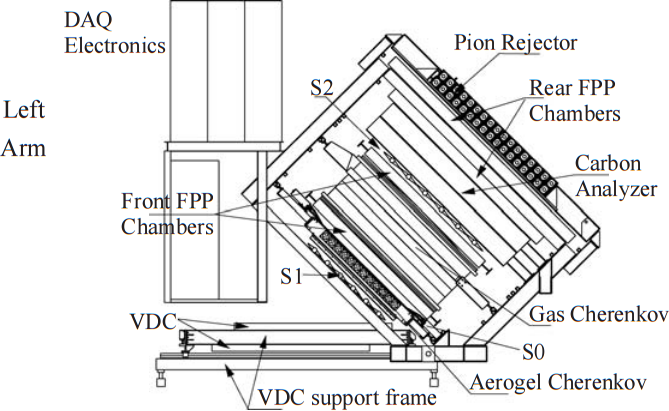
\includegraphics[width=10cm]{HRS_s.png}
	\caption{A view of both the left(top) and right(bottom) detector stacks inside the left and right HRS \cite{HallA}.
	\label{hrsss}}
\end{figure}

	\subsection{Vertical Drift Chambers}\label{sec:vdc}
	\paragraph{}Each of the spectrometers housed in Hall A contains two vertical drift chambers(VDC). Each VDC incorporates two planes of crossing sense wires. Shown in figure \ref{VDC_profile}, the two planes of the VDC lie a distance of 0.335m apart \cite{drift}. The lower plane of the VDC is positioned at the approximate focal plane of the HRS and lies in the horizontal plane of the Hall A coordinate system. The sense wires located in the VDCs cross orthogonally. They are offset by $45^\circ$ in respect to the dispersive and non-dispersive directions. Each plane of the VDC uses 368 sense wires, with 4.24 mm between each wire. The signals from these wires are transmitted to the electronics via a set of printed circuit boards that contain a 16-channel connector and twisted pair ribbon cables. These ribbon cables transmit the VDC signal to a set of common stop TDCs with 0.5 ns resolution \cite{drift}. The VDC sense wires are held at ground potential between two planes of high-voltage. Particles that enter the gas-filled VDC, collide with molecules of an argon($62\%$) and ethane ($38\%$) mixture \cite{HallA}. This collision causes the ionization of the gaseous mixture producing drift electrons.
	\begin{figure}
		\centering
		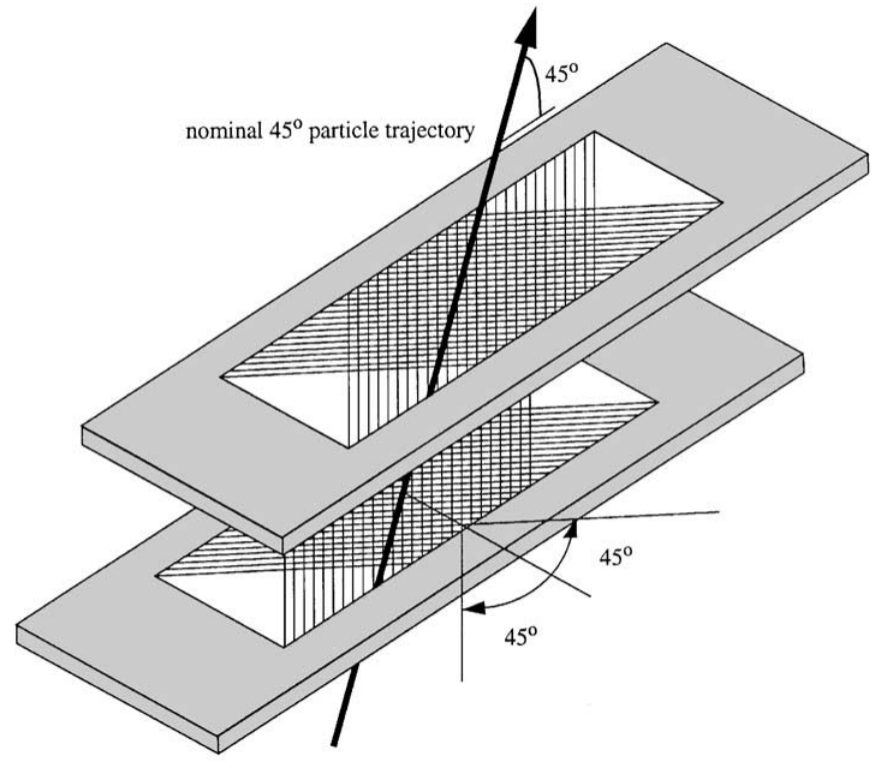
\includegraphics[width=10cm]{VDC_profile_view.png}
		\caption{A sketch of the two VDC planes in the HRSs with a particle traveling through the detector at 45$^\circ$.\cite{drift}.
			\label{VDC_profile}}
	\end{figure}
	\paragraph{} Particles that traverse the VDCs will travel through regions close to several sense wires. As the indecent particle ionizes gas in each of these regions, the VDC sense wires pick up the corresponding signal from the drift electrons. The drift electrons will travel to the sense wires via the parallel electron field lines until the electrons get close to the sense wires. Once close the sense wires, the electron field transitions to a radial field and the drift electrons then move to the sense wires. An example of a drift electron's trajectory  is shown in figure \ref{vdcpath}, where a cluster of 5 wires sense the scattered particle.
	\begin{figure}[t]
		\centering
		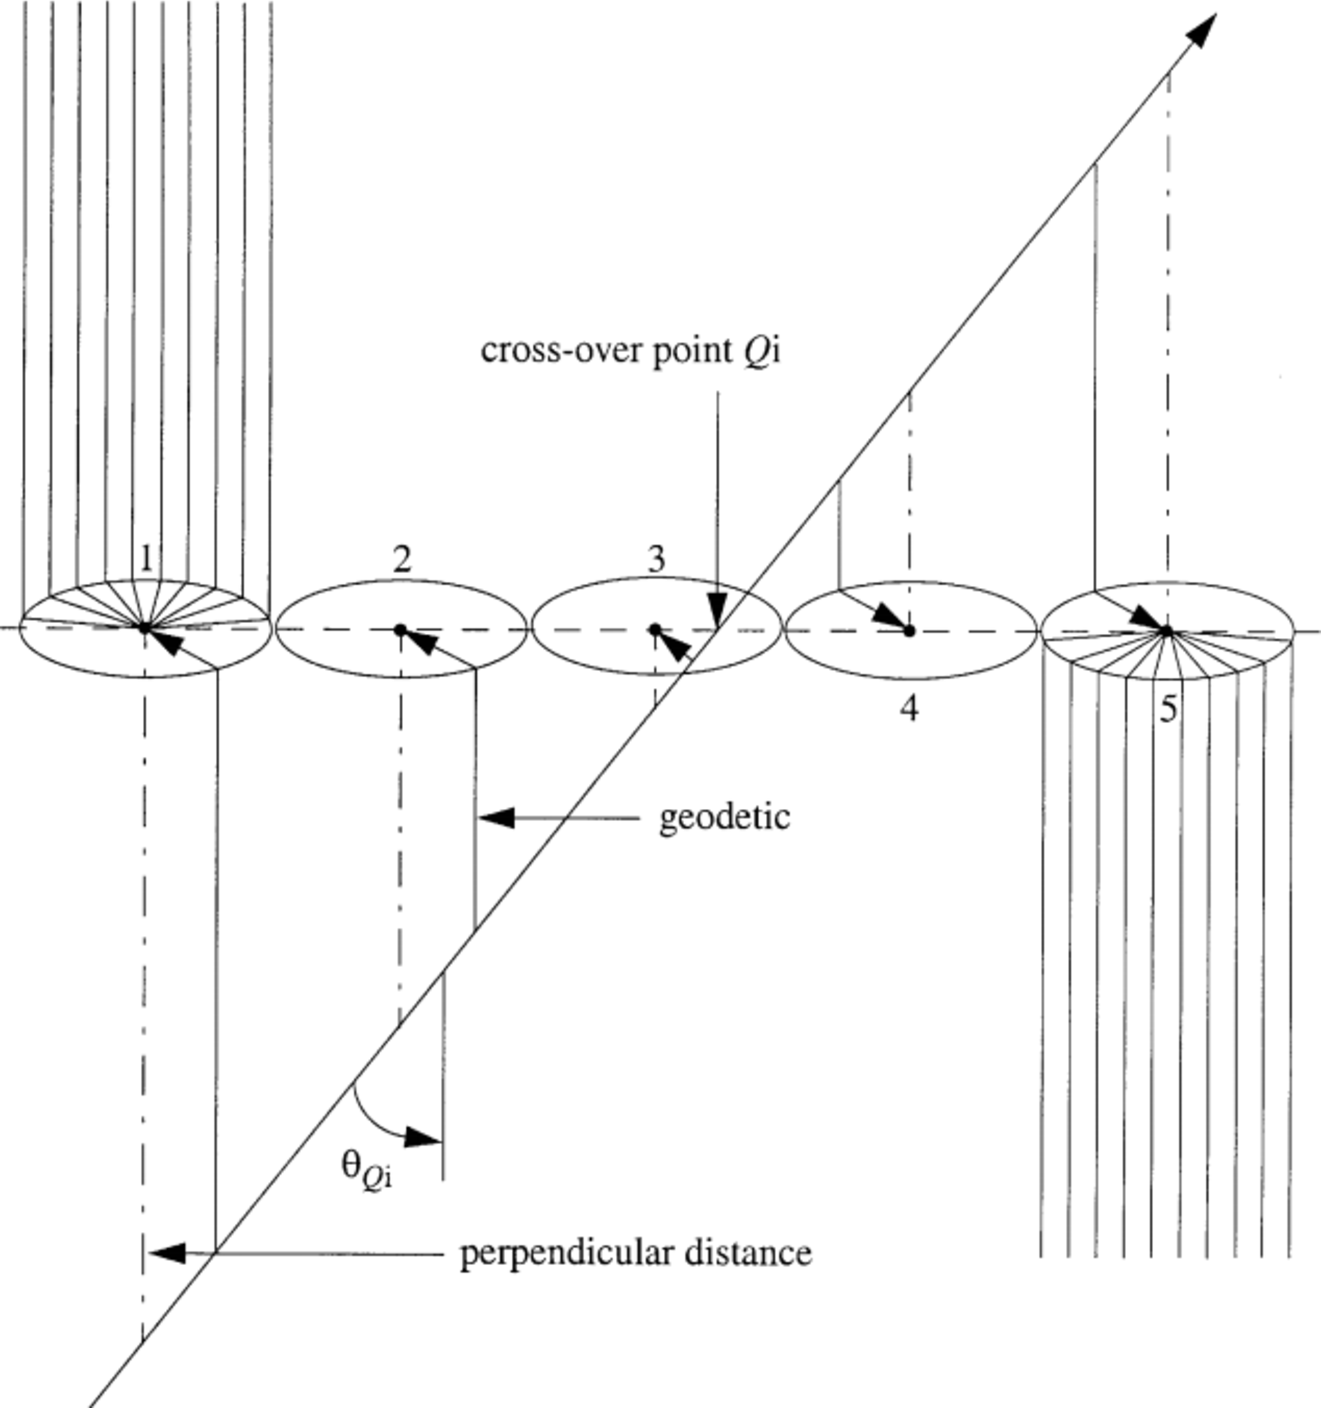
\includegraphics[width=8cm]{VDCpath.pdf}
		\caption{A possible track that causes signals in  wires. The drift electrons will follow the arrow path. The dot/dashed lines correspond to the projected distance used to reconstruct the path of the incident particle. The transition point from parallel to radial field lines is represented by the ellipses. \cite{drift} }
		\label{vdcpath}
	\end{figure}
	\begin{figure}
	\centering
	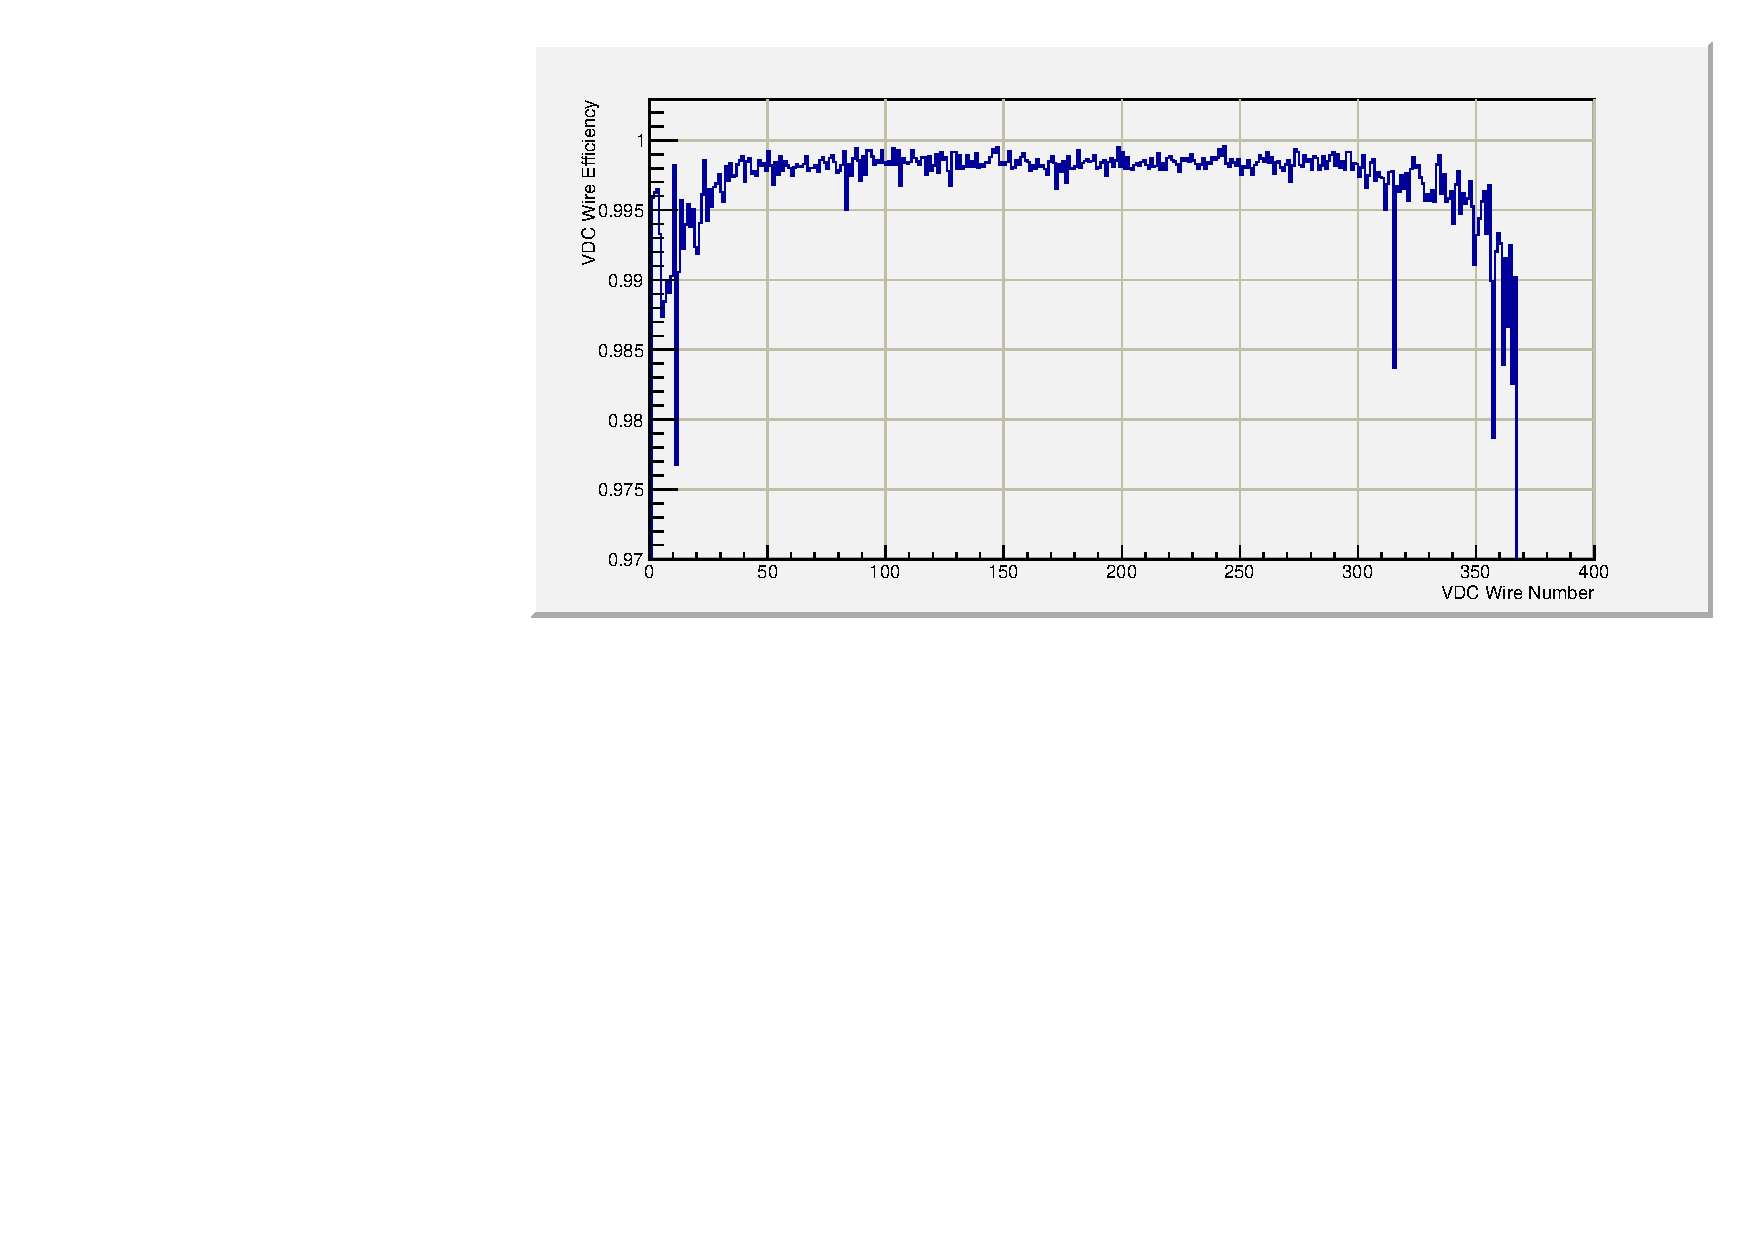
\includegraphics[width=13cm]{VDCeff.pdf}
	\caption{The VDC efficiency for one plane of wires.}
	\label{vdceff}
	\end{figure}


	\paragraph{}The drift chamber's performance is constantly monitored throughout the experiment. The efficiency of an individual wire is determine by an algorithm that scans a plane for an event that fires a cluster of wires. A wire is determined to be efficient for that event if it fired along with it's two nearest neighbors. This efficiency calculation is used during the online analysis to keep track of the performance of the VDCs and to assist in the maintenance of the HRSs throughout the experiment. 

	\paragraph{}The VDC's main task during an electron counting experiment is to determine the track of the scattered electron. The track of the electron is used to ascertain the electron's scattering momentum and scattering angle. Due to the electron's relativistic nature the primary ionization event for each wire region happens simultaneously compared to the resolution of the TDCs. The common stop TDCs used for the VDC signals record the amount of time from drift electron's signal in the sense wires to the stop signal formed by the trigger. This creates a high TDC signal for short drift distances. The raw TDC values recorded by the VDC include time associated with the signal but also the time required to form the trigger and time of flight for electrons between the VDCs and detectors used in the formation of a trigger. The calibration of the VDC removes these extra sources of time in the TDC signal. In order to calibrate the VDC raw signals, a reference time is determined for every wire on every plane. The sharp decrease on the outside of the peak in region C shown in figure \ref{fig:vdcraw} defines the references time ($t_0$) of a VDC's TDC signal.The time recorded from the TDCs is used to construct the location of an ionization event for each sense wire across the scattered electron's trajectory. The analyzing software will use these drift distance from the four VDC planes to find a track for the scattered electron.
	\begin{figure}[H]
		\centering
		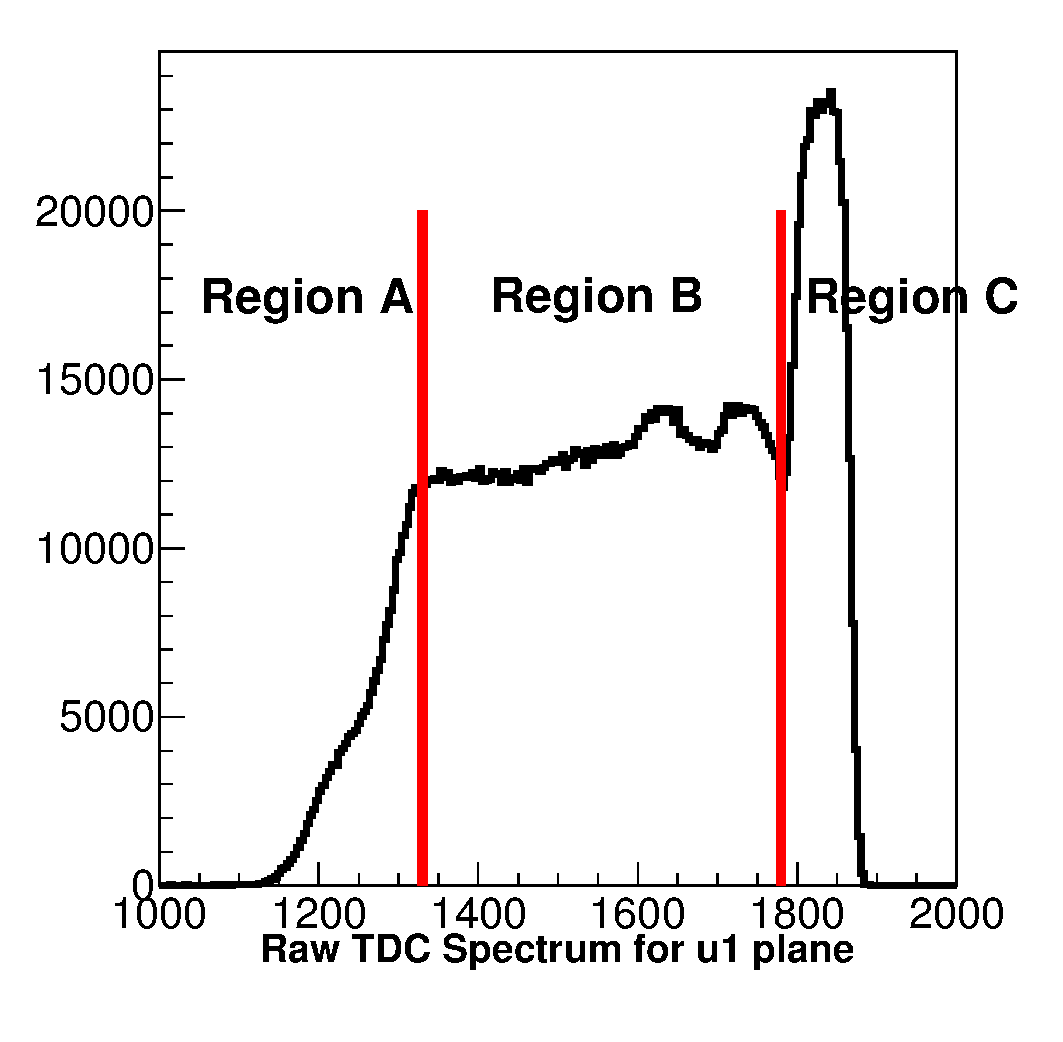
\includegraphics[width=7.5cm]{vdc_raw.pdf}
		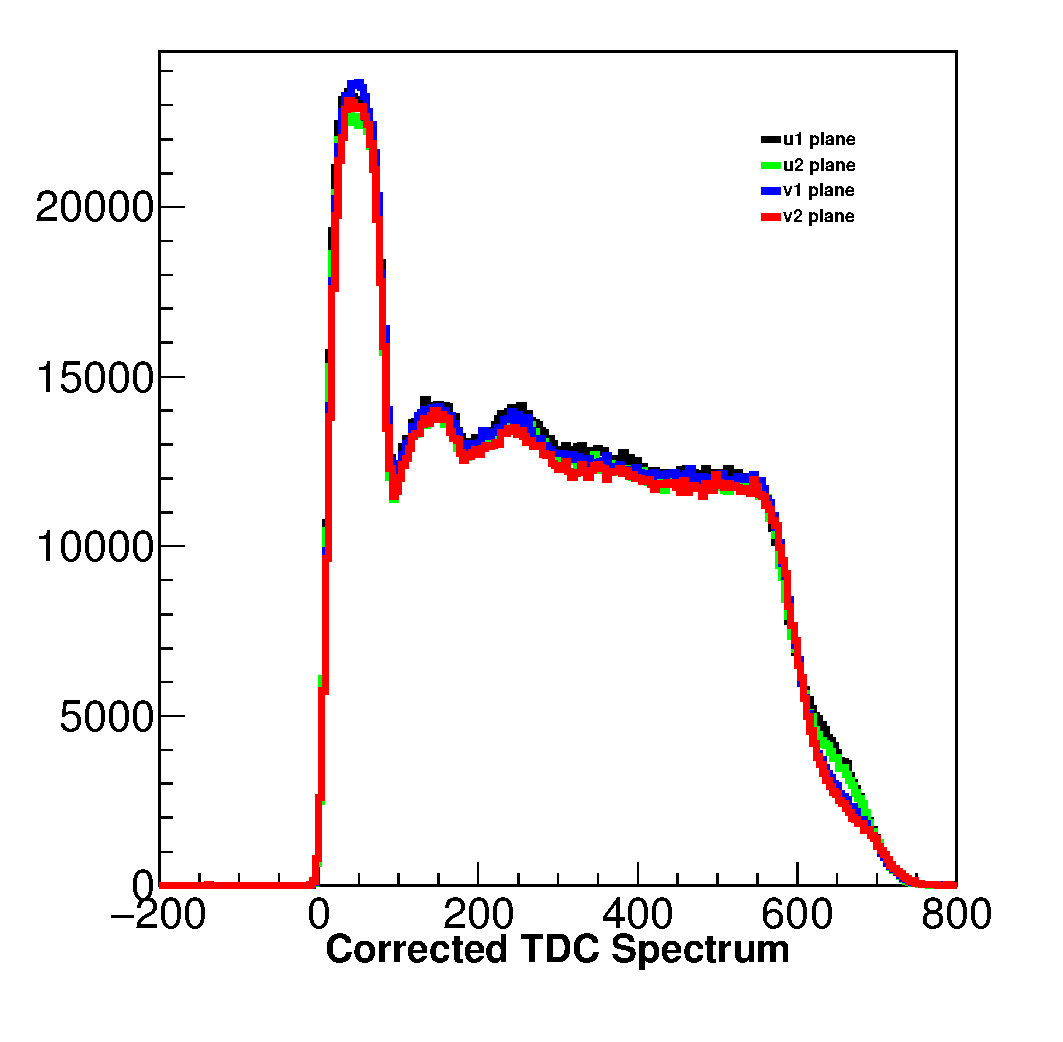
\includegraphics[width=7.5cm]{vdc_cal.pdf}
		\caption{Histograms of VDC signals before(left) and after(right) calibration of t0\cite{primer}.}
		\label{fig:vdcraw}
	\begin{itemize}
		\item Region A: In this region, the point of primary ionization is far from the sense wire. As this distance increases, the chance of detecting the traversing particles by this wire decreases. 
		\item Region B: The probability of sense wires detecting a primary ionization event in this region are uniform due to the uniform electric field though out the region. 
		\item Region C: The primary ionization position for these events are very near the sense wire and the electric field from this area is going to change to radial shape and the 	probability to detect a particle is going to increase in this area. The sense wire exist in the region, so the ionization event will have a minimum distance. This is shown in the sharp decline on the outside of the peak in region C. 
		\cite{primer}
	\end{itemize}	
	\end{figure}


	\subsection{Scintillators}\label{sec:scin}
	\paragraph{} A pair of scintillator planes form the primary triggering apparatus for the HRSs. The planes of scintillator S0 and S2 consist of a collection of plastic scintillating paddles with photo multiplier tubes(PMTs) attached to both ends of the paddle. S0 the first scintillator in the stack consist of one scintillating paddle in a vertical direction. S2, the second scintillator was built with 16 overlapping paddles with PMTs attached to both ends. As electrons enter the scintillating plastics, photons are emitted via the scintillating interaction. These photons are detected by the PMTs on either side of the scintillator bar. The passing of the electron can happen at positions at an unequal distances from the PMTs on a scintillator bar. These relative differences cause a distortion in the timing calculation in the time of flight(TOF) known as the time walk effect. The scintillators are used in the calculation of $\beta$, the relativistic $v$ to $c$ ratio. Beta is calculated using the TOF between the two scintillator planes and distance traveled between the points of interaction. 
	\begin{figure}[t]
		\centering
		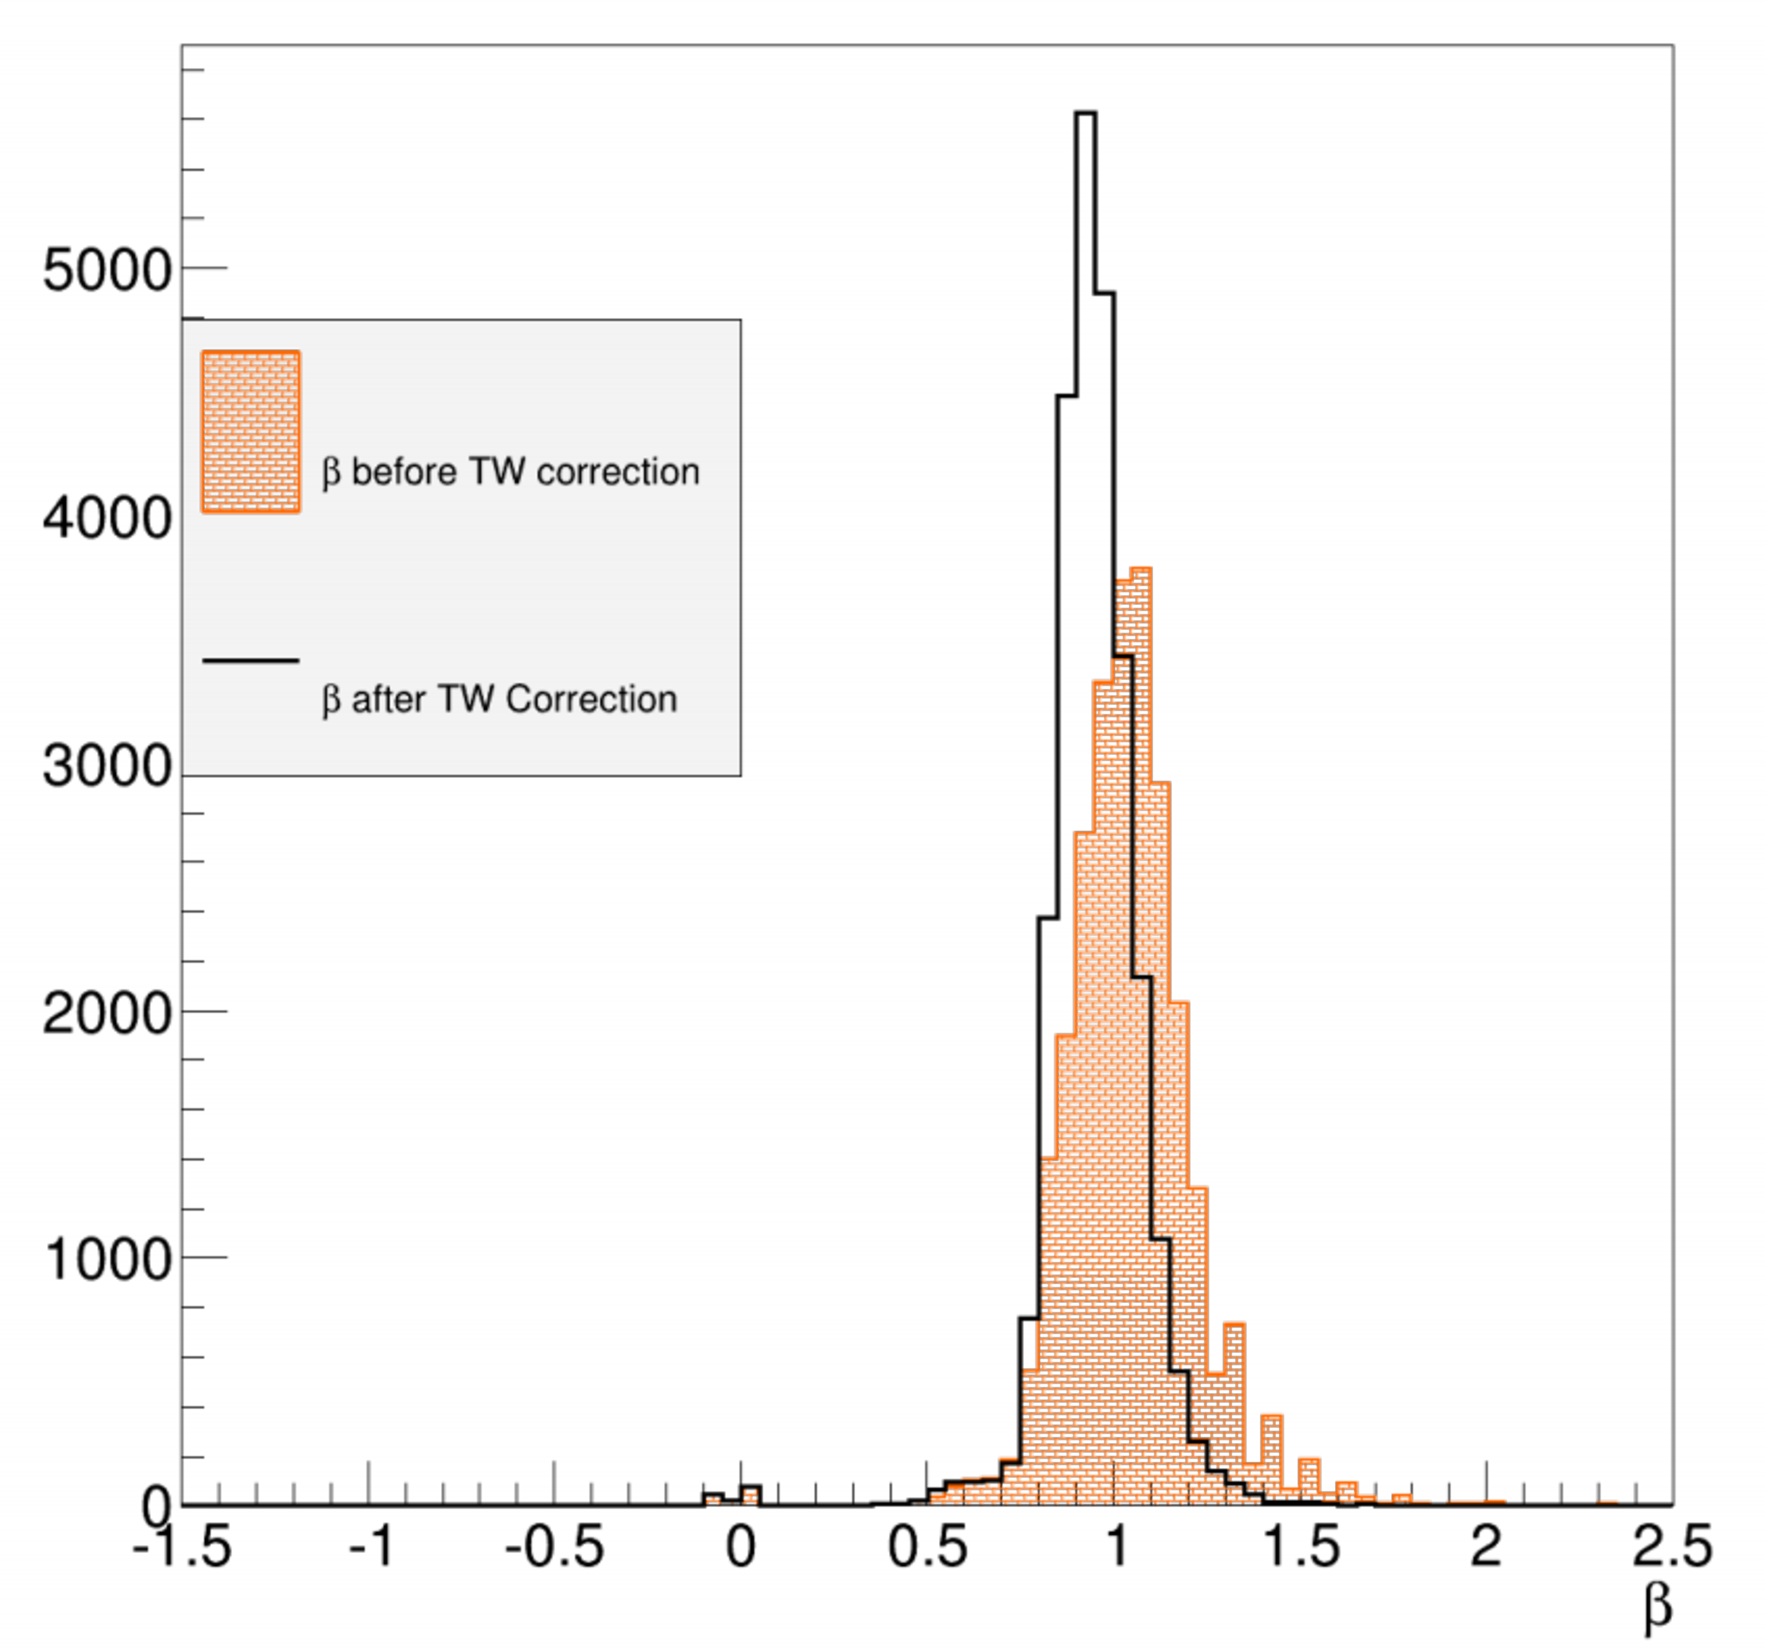
\includegraphics[width=9.5cm]{twcor.pdf}
		\caption{Histogram of $\beta$ before and after time walk correction.}
		\label{fig:twcor}
	\end{figure}
	Once calibrated, each plane has a time resolution of about 0.3 ns. This high time resolution and quick response makes the scintillators the perfect detector to form the main trigger.  
	
	\subsection{Cherenkov}\label{sec:Cer}
	\paragraph{}After a particle passes through S0, it will enter the large gas chamber for the gas Cherenkov(GC). The GC is filled with $CO_2$ with an index of refraction of 1.00041. This high index of refraction creates a momentum threshold of 0.017 GeV/C for electrons, 4.8 GeV/C for pions, and 32 GeV/c for protons\cite{GasC}. Relativistic particles entering the GC will produce a cone of Cherenkov radiation. This cone of light will be focused by a set of mirrors on the back plane of the GC. These mirrors direct the focused light onto a set of PMTs. A depiction of the GC from a top down perspective is shown in figure \ref{fig:cer_TD}. 
	\begin{figure}[t]
		\centering
		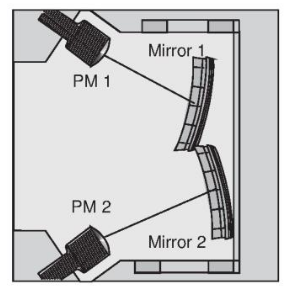
\includegraphics[width=7.5cm]{Cher.png}
		\caption{Top down depiction inside the GC \cite{GasC}.}
		\label{fig:cer_TD}
	\end{figure}
	The raw data recorded from the GC is in the form of raw ADC, or the size of the pulse seen by the PMT. In order to use this information, the ADC input needs to be calibrated. For the GC, two parts of the signal needs calibration. Each ADC channel sees a different amount of noise and signal background from electronic fluctuations. This signal background is defined as the ADC pedestal, and is the fist calibration offset determined. Figure \ref{fig:cer_raw} shows the raw signal from one Cherenkov PMT. This signal shows the pedestal at approximately 5800 ADC channels. The pedestal is subtracted from the raw ADC signal to normalize the background electronic noise for all PMT-ADC pairs in the Cherenkov. The second calibration for the GC ADC signals is the photo electron peak. The voltage used to power the PMTs in the Cherenkov is tuned before the experiment to allow the PMT to give the best pedestal to signal ratio while also persevering the life of the PMT and signal quality. This forces a different signal strength to be seen by each PMT for the same amount of light experienced in the chamber. The photo electric peak in the ADC signal is then normalized to the same value across all PMTs by a gain factor. 
	\begin{figure}[t]
		\centering
		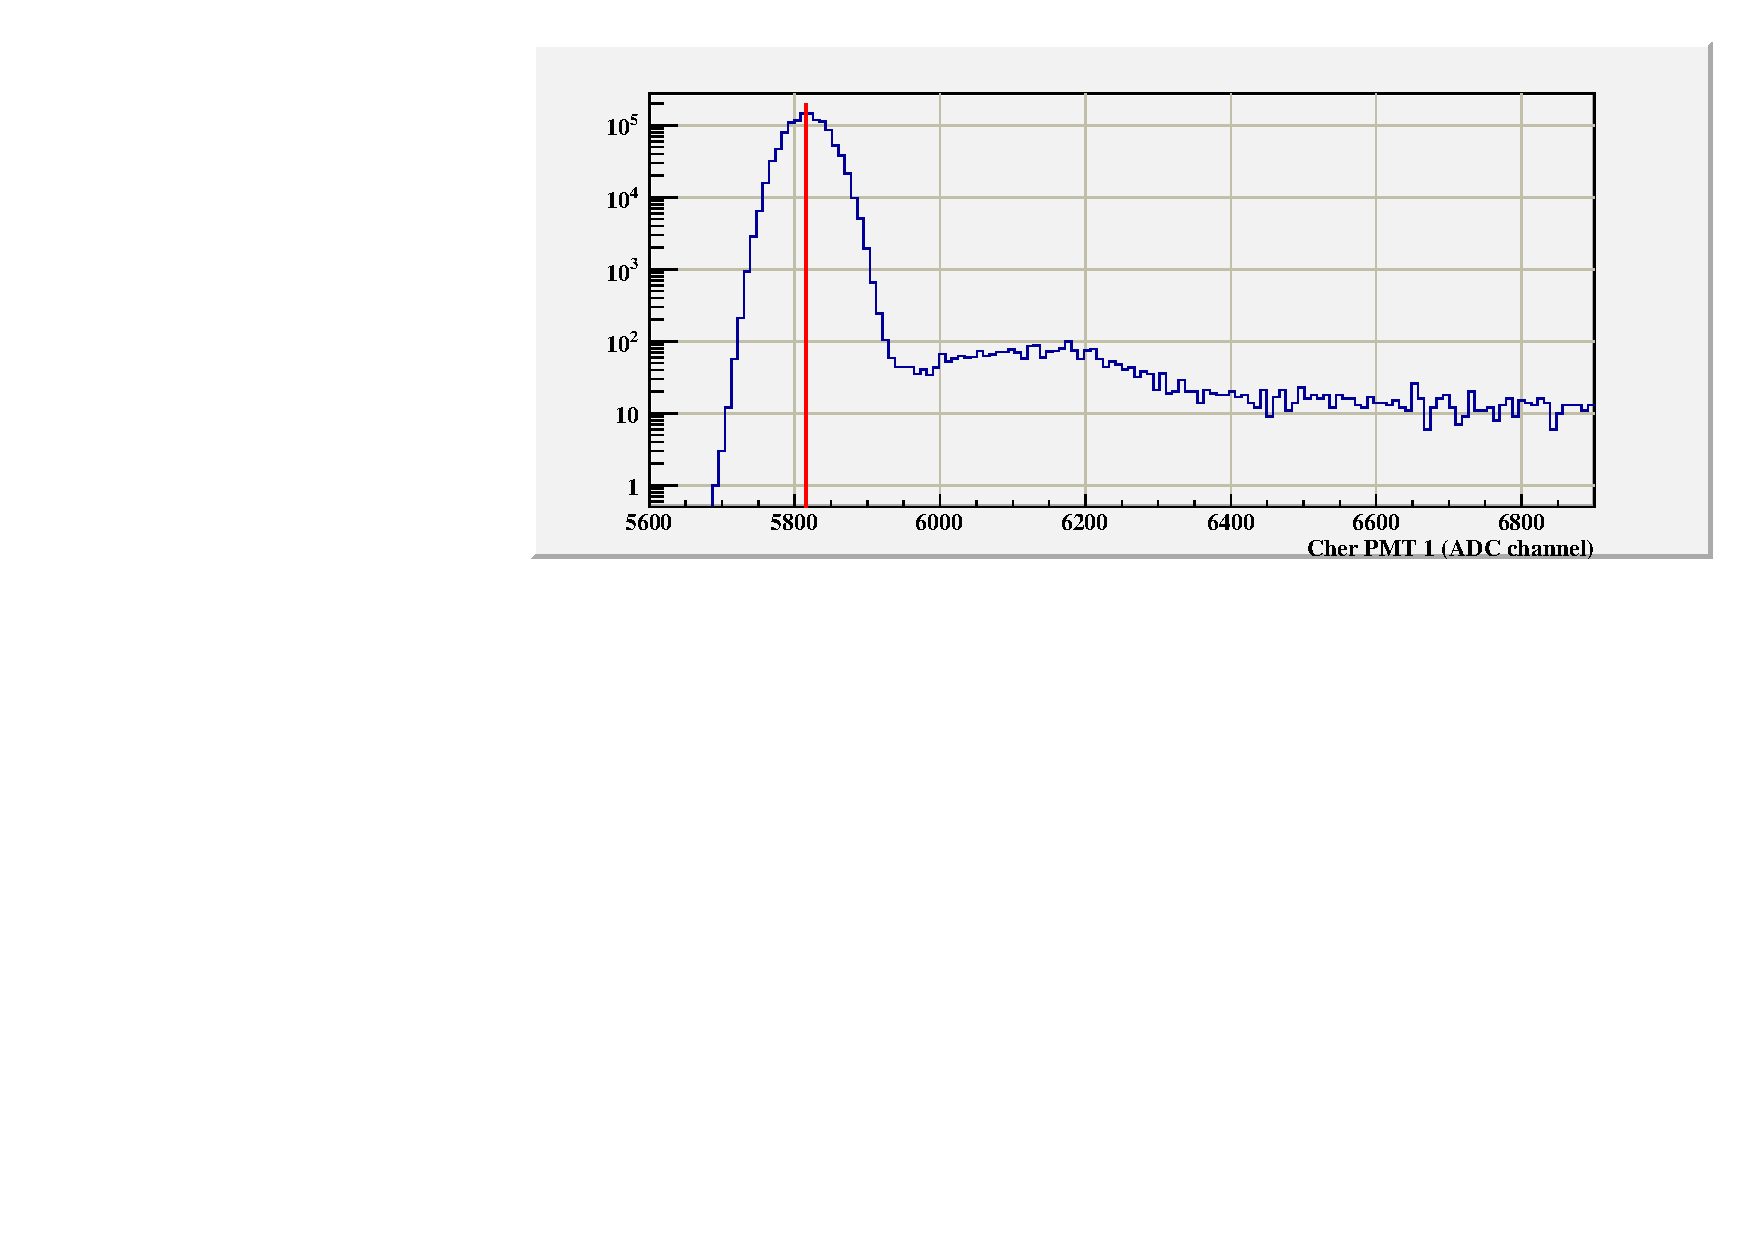
\includegraphics[width=14.cm]{Cher_raw1.pdf}
		\caption{The raw signal captured from a single Cherenkov PMT, PMT[1], with a fit to the pedestal peak and a line draw to demonstrate its ADC channel number.}
		\label{fig:cer_raw}
	\end{figure}
	\paragraph{}The GC's main task during an experiment is to help in the identification of particles(PID). During the MARATHON experiment, the GC was used to differentiate between negatively charged pions and electrons that passed through the detector. MARATHON used the GC in PID for data capture and analysis. During data capture, the GC signal was used in the formation of the main trigger. Forming the trigger with a requirement of a threshold in signal strength from the GC, allowed for the exclusion of many unwanted events. During the analysis of MARATHON data, pion suppression was done using the GC signal and signals from the calorimeter.   
	\subsection{Calorimeter}\label{sec:Cal}
	\paragraph{}The last detector in the spectrometer that particles interact with is the lead glass calorimeter. The Left HRS (LHRS) calorimeter system is made up of the preshower(PS) and shower(SH). The PS contains two columns of 24 blocks of lead glass with a PMT attached to the end. The SH has five columns, and each column as 16 blocks with a PMT. The right HRS'(RHRS) calorimeter system is constructed of the pion rejector 1(PR1) and the pion rejector 2(PR2). The two PRs on the RHRS consist of 34 blocks arranged in two, 17 block columns. 
	\paragraph{}The calorimeters are used during the analysis process to help in PID. As high energy electrons pass through the dense leaded glass, the electron will lose its energy through bremsstrahlung radiation resulting in the emission of a photon. These photons begin an electromagnetic shower through the creation of positron-electron pairs. The shower of photons are detected by the PMTs attached to each block. The amount of energy contained in the scattered electron is directly proportional to the amount of photons generated during the shower.
	\paragraph{} The signal from the calorimeters is recorded as an ADC value. These ADC signals need to be calibrated similar to the Cherenkov detector, subtracting the pedestal and determining the normalizing gain factor to match all PMT-ADC combinations. The total signal seen from the colorimeter can be seen in figure \ref{fig:calo_raw}. In order to use this ADC signal to help ID particles, the calorimeter needs an energy calibration. 
	\begin{figure}[t]
		\centering
%		\hspace*{-65pt}
		\subfloat[ADC Sum]{
		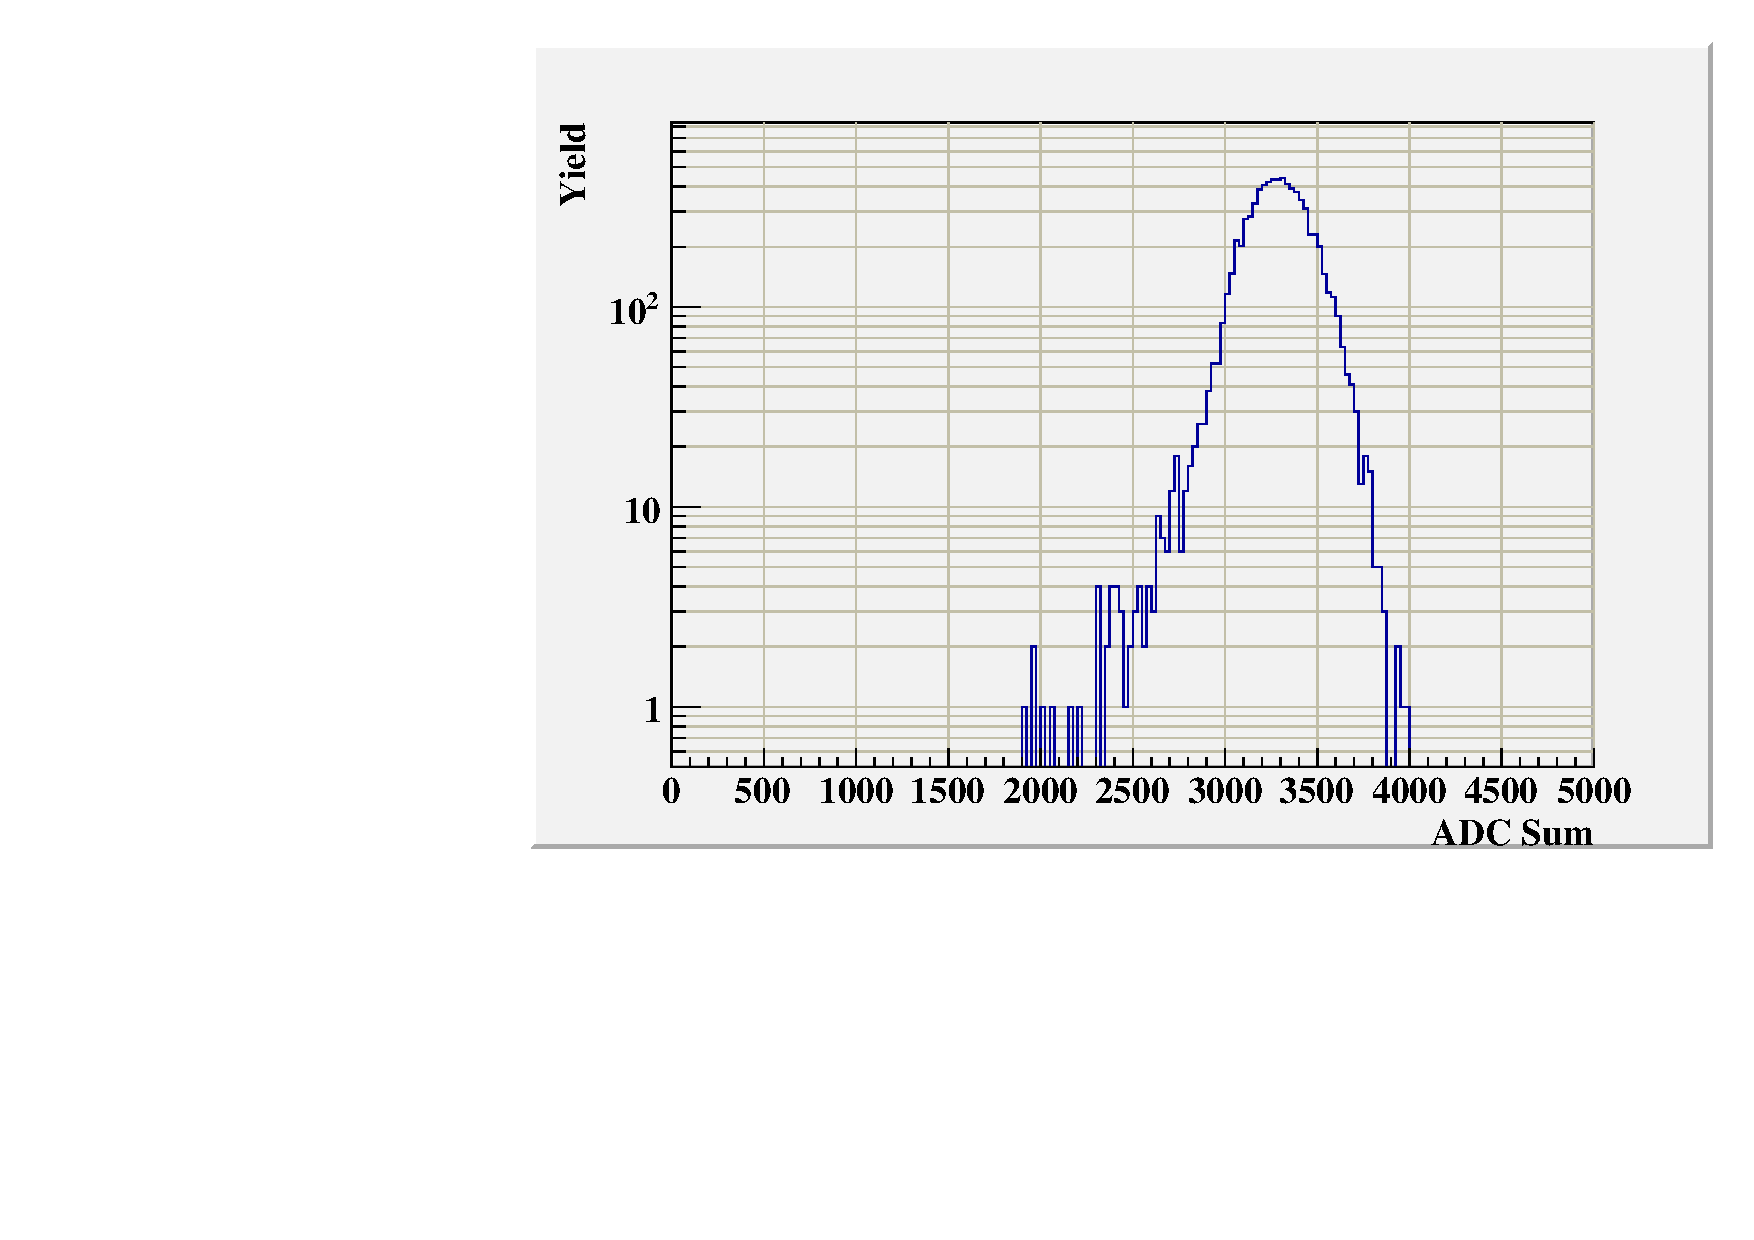
\includegraphics[width=7.25cm]{calo_adcs.pdf}
		\label{fig:calo_raw}}
		\centering	
		\subfloat[$E^\prime / P$]{
		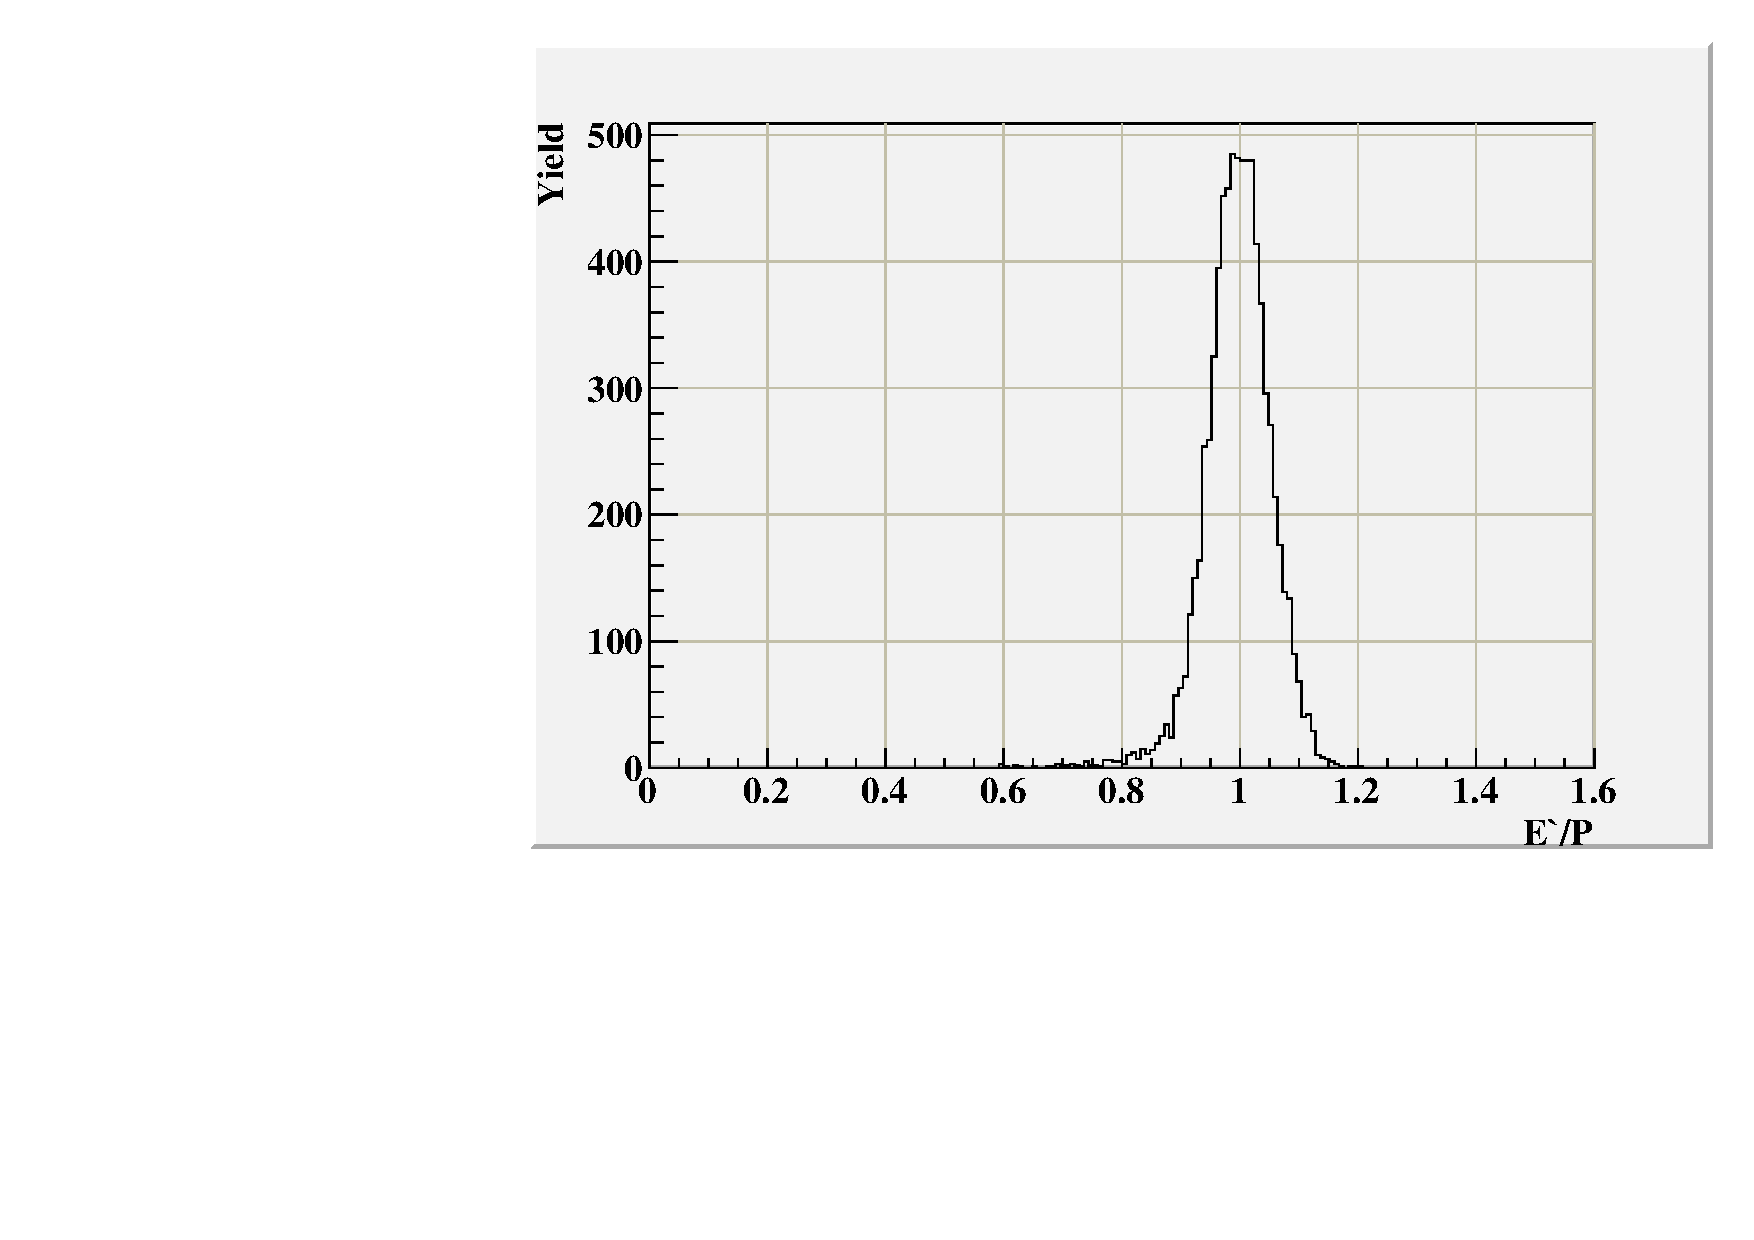
\includegraphics[width=7.25cm]{calo_ep.pdf}
		\label{fig:calo_ep}}
		\caption{Left: The sum of all ADC channels from the LHRS calorimeters. Right: The total energy deposited into the LHRS calorimeter scaled by the momentum setting. Electron cuts have been applied.}
	\end{figure}
	The calibration process uses a $\chi^2$ minimization. Equation \ref{EQ:cal_cal} demonstrates the minimization technique applied. In this equation, $C_j$ is the calibration coefficient being determined for the calorimeter block j. $Cal^{ADC}_{ij}$ is the ADC signal received from block j during event i, and $p_i$ is the momentum of the electron being detected. 
	\begin{equation}
		\frac{\partial\chi^2}{\partial C_i} = \sum\limits_{i}^{Events} \bigg( \sum\limits_{j}^{Blocks}C_{j}*Cal^{ADC}_{ij} - p_i  \bigg)^2 = 0 
		\label{EQ:cal_cal}
	\end{equation}
	Using these calibration constants, the ADC signal in figure \ref{fig:calo_raw} can be turned in the calibrated data in the histogram show in figure \ref{fig:calo_ep}. This can be used to from PID selection cuts, removing any unwanted background events.  
	
\section{Trigger Setup}\label{sec:Trig}
\paragraph{} The MARATHON experiment designed three triggers to accept the most probable good electron events, while limiting the number of background events and preventing loss of efficiency due to electronic dead time. The design of these trigger are depicted in figure \ref{fig:trig_layout}. Each trigger is built by the coincidence of signal between S0, S2 and the gas Cherenkov.  Trigger 1(T1) is the logical $\&$ between the S0 and S2. This is used as a loose trigger to help test the detector timing and efficiencies.  Trigger 2(T2) is the main trigger used for good electron selection for the MARATHON experiment and is by  combining T1 and GC with a logical $\&$. The addition of the GC helps remove many background pions and cosmic rays compared to T1. Trigger 3(T3), a logical $||$ between S0 and S2 and $\&$ with the GC, was designed to help with the study of the efficiency of T1 and T2. The RHRS uses the same triggers, T4 copy of T1, T5 copy of T2, and T6 copy of T3.
\begin{figure}[t!]
%	\hspace*{-2cm} 
	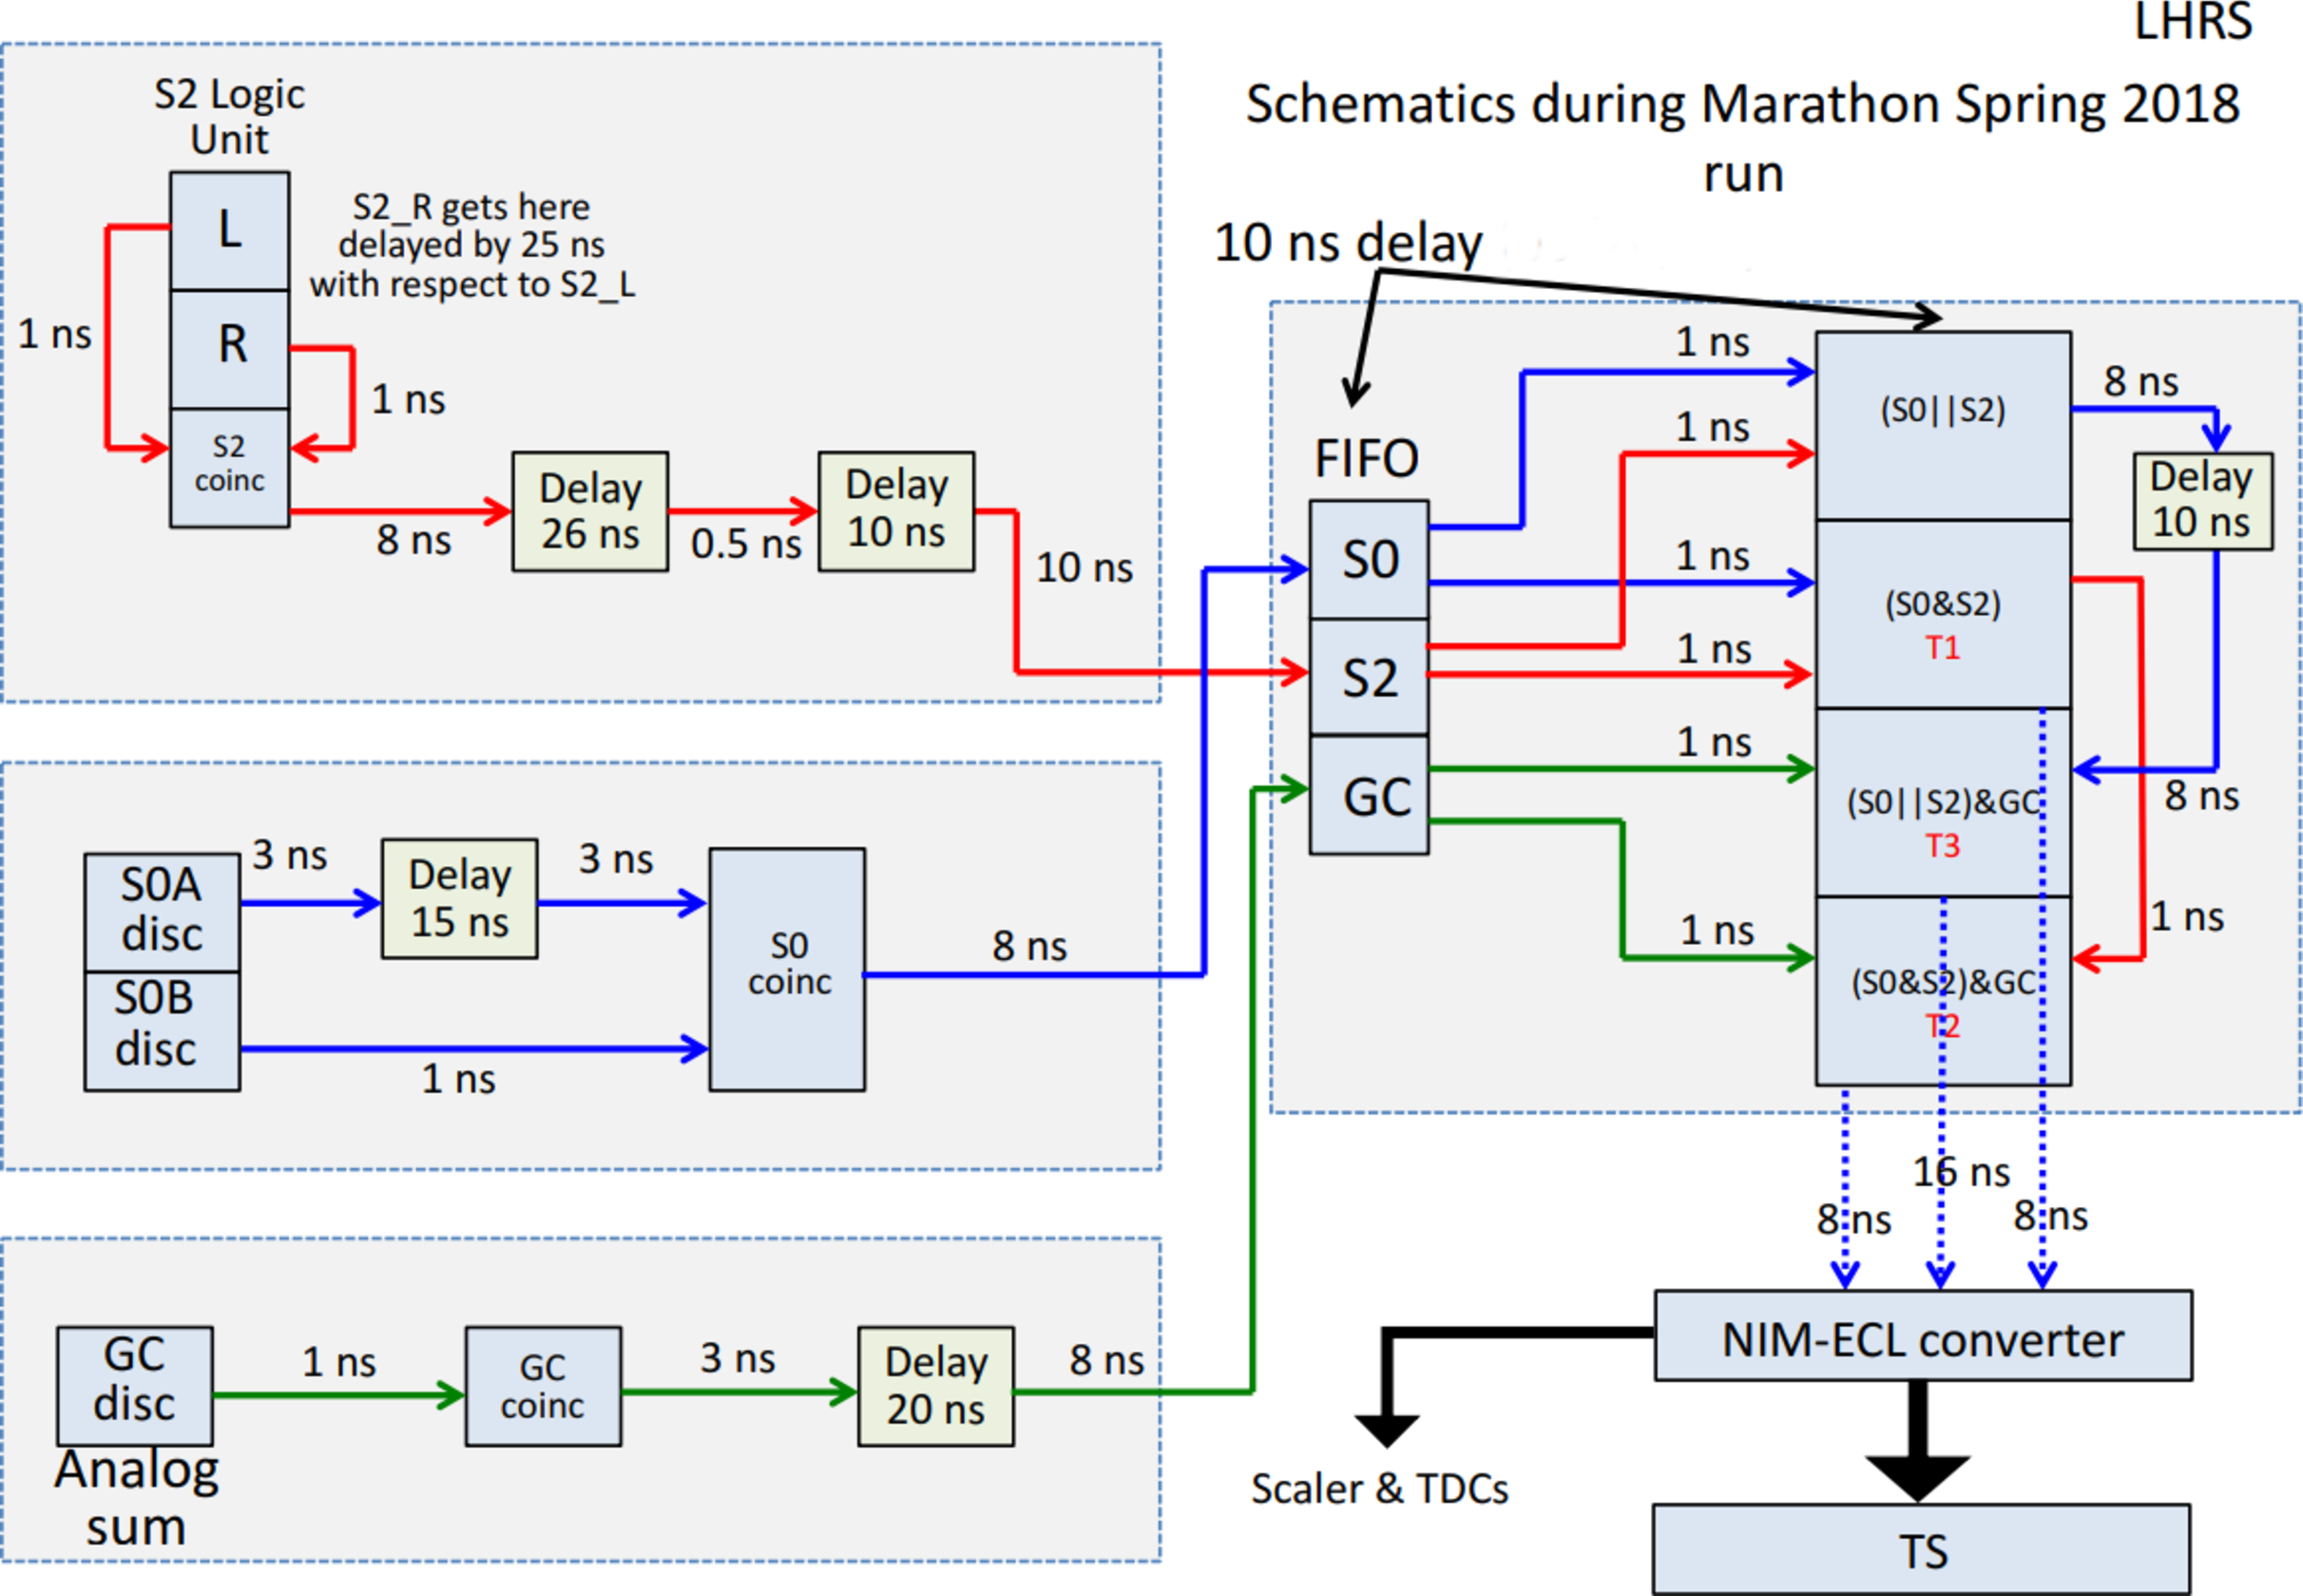
\includegraphics[width=14.5cm]{trigger_layout.pdf}
	\caption{Scematic drawing of the trigger logic and timing for the MARATHON experiment \cite{flo_trig}.}
	\label{fig:trig_layout}
\end{figure}
\paragraph{}The trigger signal from  S0 is the logical and between the signals of the two PMTS of S0. S0A has an additional time delay. This delay forces the leading edge of S0B to be the leading edge of the output of the S0 coincidence. The trigger signal for S2 is built by a coincidence in both the left and right PMT attached to each bar of the scintillator. The signal from the right PMT is used as the leading edge of the coincidence signal. S2 has many bars so the trigger source is formed by a coincidence in any of the S2 scintillator bars. The S2 trigger signal has an additional delay compared to the S0 trigger signal. This delay forces S2R to be the leading edge of all the logical $\&$ triggers The GC signal is formed by a sum of all the PMTs in the GC. If this sum meets some discriminator threshold, a trigger signal from the GC will be formed. The signals formed from the logic units for each of these trigger signals receive additional delays to prefect their timing in respect to each other. This tweaking of the timing spreads the trigger signals apart to help prevent the trigger signals from overlapping and allowing the recording of all possible triggers. 
 
%\section{DAQ - Data Acquisition System}\label{sec:daq}

\section{Kinematic Settings}\label{sec:kin}
\paragraph{} The MARATHON experiment's goal is to study cross section ratios of $^3$H, $^3$He, $^2$D, and H. as a function of $X$. The MARATHON collaboration originally proposed to use the kinematics in table \ref{OldKT}, allowing for the LHRS and RHRS to have mirror settings to expedite the rate of data collection at each position of $X$. The plan was to complete one kinematic setting and push the spectrometers out in angle from near 18 degrees at kinematic 1 to near 35 degrees at kinematic 16 while keeping the momentum settings of the spectrometers at 3.10 GeV for the 1st 15 settings, then decreasing the momentum to 2.9 for the last kinematic. 

\begin{table}[t]
		\caption{Kinematics originally planned for the MARATHON experiment inlcuding an estimation of time required for three of the gas targets in hours. Estimations provided by John Arrington and Zhihong Ye\cite{RateEst}. }
	\label{OldKT}
	\begin{tabular}{|l|l|l|l|l|l|l|l|l|l|}
		\hline
		Kin. & $X_{Bj}$& W2    & Q2    & E$^\prime$    & Theta & H2   & H3   & He3   & Total  \\ 
        &&Ge$V^2$&Ge$V^2$& GeV & Degree& (h)& (h)&(h)&(h)  \\ \hline
		1    & 0.23 & 12.30 & 3.41  & 3.10 & 18.19 & 0.28 & 0.45 & 0.28  & 1.02   \\ \hline
		2    & 0.27 & 11.70 & 4.00  & 3.10 & 19.73 & 0.42 & 0.69 & 0.43  & 1.54   \\ \hline
		3    & 0.31 & 11.11 & 4.60  & 3.10 & 21.15 & 0.62 & 1.03 & 0.62  & 2.27   \\ \hline
		4    & 0.35 & 10.52 & 5.19  & 3.10 & 22.49 & 0.90 & 1.50 & 0.89  & 3.29   \\ \hline
		5    & 0.39 & 9.92  & 5.78  & 3.10 & 23.76 & 1.29 & 2.17 & 1.27  & 4.73   \\ \hline
		6    & 0.43 & 9.33  & 6.37  & 3.10 & 24.97 & 1.85 & 3.13 & 1.81  & 6.79   \\ \hline
		7    & 0.47 & 8.74  & 6.97  & 3.10 & 26.12 & 2.66 & 4.52 & 2.57  & 9.75   \\ \hline
		8    & 0.51 & 8.14  & 7.56  & 3.10 & 27.23 & 3.80 & 6.53 & 3.66  & 13.99  \\ \hline
		9    & 0.55 & 7.55  & 8.15  & 3.10 & 28.30 & 5.52 & 9.56 & 5.27  & 20.36  \\ \hline
		10   & 0.59 & 6.96  & 8.75  & 3.10 & 29.34 & 5.12 & 14.19& 7.70  & 30.01  \\ \hline
		11   & 0.63 & 6.37  & 9.34  & 3.10 & 30.34 & 12.12& 21.39& 11.41 & 44.92  \\ \hline
		12   & 0.67 & 5.77  & 9.93  & 3.10 & 31.31 & 18.56& 33.08& 17.35 & 68.99  \\ \hline
		13   & 0.71 & 5.18  & 10.53 & 3.10 & 32.26 & 29.08& 52.35& 26.98 & 108.41 \\ \hline
		14   & 0.75 & 4.59  & 11.12 & 3.10 & 33.18 & 47.19& 85.80& 43.47 & 176.46 \\ \hline
		15   & 0.79 & 3.99  & 11.71 & 3.10 & 34.08 & 87.73&150.03& 74.76 & 306.51 \\ \hline
		16   & 0.83 & 3.40  & 12.30 & 3.10 & 34.96 &155.36&287.74&141.21 & 584.30 \\ \hline
	\end{tabular}
\end{table}

\begin{table}[t]
	\caption{Kinematic settings used during the MARATHON experiment. Kinematic 1-15 for LHRS, and kinematic 16 using RHRS. The good electron count is in units of thousands. }
	\label{newkin}
	\begin{tabular}{|l|l|l|l|l|l|l|l|l|}
		\hline
		kin & X    & W2    & Q2    & E`   & theta & D2 count & He3 count & H3 count \\ \hline
		1   & 0.22 & 11.89 & 3.07  & 3.1  & 17.58 & 94.0   & 93.0      & 124.3    \\ \hline
		2   & 0.26 & 11.33 & 3.62  & 3.1  & 19.11 & 109.0  & 103.0     & 120.5    \\ \hline
		3   & 0.3  & 10.76 & 4.19  & 3.1  & 20.58 & 121.0  & 78.0      & 101.1    \\ \hline
		4   & 0.34 & 10.2  & 4.76  & 3.1  & 21.93 & 78.0   & 64.0      & 69.8     \\ \hline
		5   & 0.38 & 9.63  & 5.32  & 3.1  & 23.21 & 25.0   & 39.0      & 39.3     \\ \hline
		7   & 0.46 & 8.51  & 6.45  & 3.1  & 25.59 & 40.0   & 40.0      & 41.2     \\ \hline
		9   & 0.54 & 7.38  & 7.57  & 3.1  & 27.78 & 36.0   & 36.0      & 35.5     \\ \hline
		11  & 0.62 & 6.2   & 8.76  & 3.1  & 29.92 & 29.0   & 27.0      & 27.6     \\ \hline
		13  & 0.7  & 5.13  & 9.82  & 3.1  & 31.73 & 23.0   & 23.0      & 23.0     \\ \hline
		15  & 0.78 & 4.0   & 10.96 & 3.1  & 33.56 & 21.0   & 23.0      & 22.8     \\ \hline
		16* & 0.82 & 3.51  & 11.82 & 2.90 & 36.12 &24.2    &23.9	   & 24.6 \\ \hline
	\end{tabular}
\end{table}

\paragraph{}Due to time and physical constraints caused by issues with the running of all four halls simultaneously, the kinematics were adjusted to provided the best chance of reaching the statical goals at a large range in $X$. The angle setting for each kinematic were adjusted slightly. Most kinematics experience a slight degrees in angle setting to increase the rate of electron counting. During the first few days of running the MARATHON experiment the RHRS dipole experience a power supply failure. This issue could not be resolved quickly. In order to complete our goal, the MARATHON experiment adjusted the kinematic plan to remove RHRS from running. The statical precision goal of the MARATHON experiment forced the collaboration to remove a few kinematic points from the plan. The kinematics that the MARATHON experiment was able to complete are listed in table \ref{newkin}. Figure \ref{fig:kincov} shows the kinematic coverage of the spectrometer for $x$, theta, and Q$^2$ for the kinematics covered during the MARATHON experiment. After the new plan was solidified and data for the first few kinematics where complete, the RHRS was restored to services. The RHRS was then set to kinematic 16 for rest of the experiment.      

\begin{figure}[t!]
%	\hspace*{-2.cm} 
	\centering
	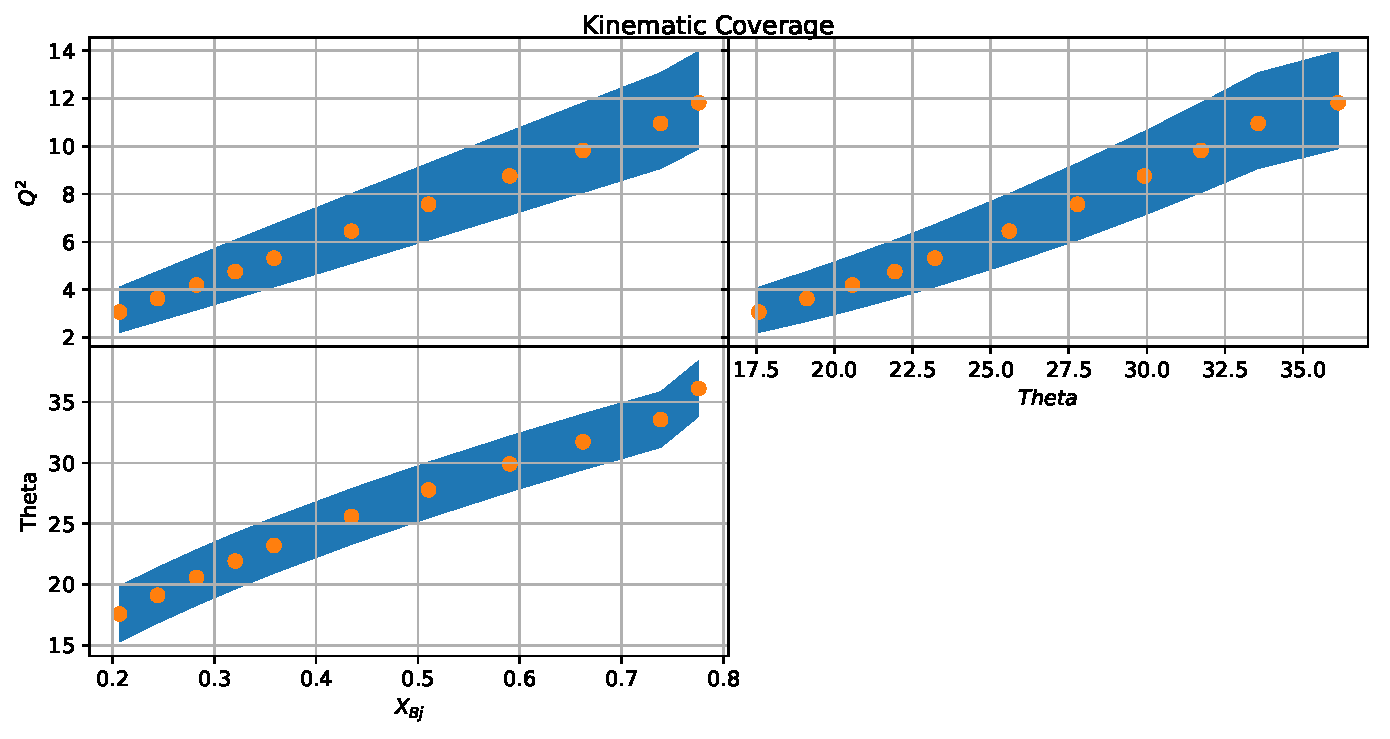
\includegraphics[width=15.5cm]{KinCov.pdf}
	\caption{A kinematic coverage plot, demonstrating the $Q^2$ coverage for $x$ and Theta. Also the relationship between $x$ and Theta. The band around the points represents the approximate spectrometer acceptance in the y axis.}
	\label{fig:kincov}
\end{figure}